\documentclass{beamer}

% Russian-specific packages
%--------------------------------------
\usepackage[T2A]{fontenc}
\usepackage[utf8]{inputenc}
\usepackage[russian]{babel}

\hypersetup{
    unicode=true % otherwise get "Glyph not defined"
}
%--------------------------------------

% Asymptote for pictures
%--------------------------------------
\usepackage{asymptote} %% comes with options inline and attach
%--------------------------------------


% graphicx for graphs
%--------------------------------------
\usepackage{graphicx}
\usepackage{subfig}
\graphicspath{
    {./pic/}
}
%--------------------------------------

% to align includegraphics
%--------------------------------------
% \usepackage[export]{adjustbox}
%--------------------------------------


\usetheme{default}

% ----------
% ----------
% ----------
% ----------
% ----------
% ----------
% CUSTOM STUFF
% ----------
% ----------
% ----------
% ----------
% ----------
% ----------
% \ddfrac command to show big fractions, not cramped up
% https://tex.stackexchange.com/questions/173899/
%--------------------------------------
\newcommand\ddfrac[2]{\displaystyle\frac{\displaystyle #1}{\displaystyle #2}}
%--------------------------------------

% \vsp command to make a spacey newline
% useful for equations arrays
%--------------------------------------
\newcommand\vsp[1][10]{\\[#1pt]}
%--------------------------------------

% partial derivatives (can \usepackage{physics}, but only one command so far, so no)
%--------------------------------------
\newcommand\pd[2]{\frac{\partial #1}{\partial #2}}
\newcommand\ddpd[2]{\ddfrac{\partial #1}{\partial #2}}
\newcommand\ddt[1]{\frac{d #1}{dt}}
\newcommand\ddddt[1]{\ddfrac{d #1}{dt}}
%--------------------------------------

% unbreakable space parenthesized reference
%--------------------------------------
\newcommand\upr[1]{~(\ref{#1})}
%--------------------------------------

% Nice letters
%--------------------------------------
\newcommand\M[0]{\mathcal{M}} % Matrix of intertia
\newcommand\AntiU[0]{\mathcal{U}} % Helper antisymmetric matrix for eqs' RHS
\newcommand\Rhs[0]{\mathcal{R}} % RHS
\newcommand\Prhs[0]{\mathcal{P}} % The family of matrices for RHS
\newcommand\prhs[0]{\mathbf{p}} % Poisson brackets
%--------------------------------------

% Tilde (proportional, approx)
%--------------------------------------
\usepackage{textcomp}
\newcommand{\textprop}{\raisebox{0.5ex}{\texttildelow}}
%--------------------------------------

\renewcommand{\vec}[1]{\boldsymbol{\mathbf{#1}}}

\newtheorem{stmt}{Утверждение}
\newtheorem{prblm}{Затруднение}

\definecolor{Periwinkle}{HTML}{4444AC}
% ----------
% ----------
% ----------
% ----------
% ----------
% ----------
% END OF CUSTOM STUFF
% ----------
% ----------
% ----------
% ----------
% ----------
% ----------

\title{Движение симметричного экипажа \\с массивными роликами на омни-колесах}

\author{К.В. Герасимов, А.А. Зобова}

\institute[мех-мат МГУ]
{
  Кафедра теоретической механики и мехатроники\\
  Механико-математический факультет\\
  МГУ им. М.В. Ломоносова
}

\date{Научный семинар имени В.В.Румянцева, Октябрь 2017}

% Delete this, if you do not want the table of contents to pop up at
% the beginning of each subsection:
\AtBeginSubsection[]
{
  \begin{frame}<beamer>{План}
    \tableofcontents[currentsection,currentsubsection]
  \end{frame}
}

% Let's get started
\begin{document}

\begin{frame}
  \titlepage
\end{frame}

\begin{frame}{План}
  \tableofcontents
  % You might wish to add the option [pausesections]
\end{frame}


\section{Постановка задачи}

\begin{frame}{Постановка задачи}{Рисунки}
    \begin{figure}
        \centering
        % \flushleft
        \minipage{0.6\textwidth}
            \asyinclude{pic_cart.asy}
            \caption{Экипаж}
        \endminipage
        % \flushright
        \minipage{0.4\textwidth}
            \asyinclude{pic_wheel.asy}
            \caption{Колесо}
        \endminipage
    \end{figure}
\end{frame}

\begin{frame}{Постановка задачи}{Тела, связи, степени свободы}
  \begin{itemize}
  \item {
    Экипаж состоит из платформы, $N$ колес и $n$ роликов,\\
    количество твердых тел:
    $$1 + N(n+1)$$
  }
  \item{
    Оси и центры колес и роликов неподвижны относительно\\
    платформы и колес соответственно
  }
  \item {
    Скорость точек контакта равна нулю:
    $$\vec{v}_{C_i} = 0, i = 1\dots N$$
  }
  \item{
    Количество степеней свободы:
    $$3 + N(n-1)$$
  }

  \end{itemize}
\end{frame}

\begin{frame}{Постановка задачи}{Координаты, псевдоскорости, связи}
  \begin{itemize}
  \item {
    Обобщенные координаты: \\
    $q = (x, y, \theta, \chi_i, \phi_k, \phi_s),$ где $i,k = 1\dots N$, $s$ -- ролики вне контакта.
  }
  \item{
    Псевдоскорости:\\
    $\nu = (\nu_1, \nu_2, \nu_3, \nu_s), \vec{v}_S = R\nu_1\vec{e}_\xi + R\nu_2\vec{e}_\eta, \nu_3 = \Lambda\dot{\theta}, \nu_s = \dot{\phi}_s$
  }
  \item {
    Связи:
	$$ \dot{x} = R \nu_1\cos\theta-R\nu_2\sin\theta, \hspace{15pt} \dot{y} = R\nu_1\sin\theta+R\nu_2\cos\theta,$$
	$$\dot{\theta} = \frac{\nu_3}{\Lambda}, \hspace{15pt} \dot{\chi}_i = \frac{R}{l}(\nu_1\sin\alpha_i - \nu_2\cos\alpha_i - \frac{\nu_3}{\Lambda}), $$
	$$ \dot{\phi_k} = \frac{R}{l\cos\chi_k-r}(\nu_1\cos\alpha_k + \nu_2\sin\alpha_k), \hspace{15pt} \dot{\phi}_s = \nu_s $$
  }

  \end{itemize}
\end{frame}

\section{Уравнения движения}

\subsection{Кинетическая энергия и лагранжиан}

\begin{frame}{Кинетическая энергия и лагранжиан}
  \begin{itemize}
  \item {
    Присутствует аддитивный член, пропорциональный $B$ -- моменту инерции ролика относительно его оси собственного вращения:
    $$ 2T = 2L = M\vec{v}_S^2 + I_S\dot{\theta}^2 + J\sum_i\dot{\chi}_i^2 + $$
    $$ + \alert{B\sum_{i,j}(\dot{\phi}_{ij}^2 + 2\dot{\theta}\sin(\kappa_j + \chi_i)\dot{\phi}_{ij})}, $$
    $$ M = \mathring{M} + Nnm $$
    $$ I_S = \mathring{I_S} + N\cdot n(\frac{A+B}{2} + mR^2 + \frac{mr^2}{2}), $$
    $$ J = \mathring{J} + n(A + mr^2) $$
  }

  \end{itemize}
\end{frame}

\begin{frame}{Кинетическая энергия и лагранжиан}
  \begin{itemize}
  \item {
    С учетом связей:
    $$ 2L^{*} = \mathring{\nu}^T \mathring{V}^T \mathring{M} \mathring{V} \mathring{\nu} + $$
    $$ + \alert{B}\sum_{i}(
    	\frac{(\nu_2\sin\alpha_i+\nu_1\cos\alpha_i)^2R^2}
    	{\rho_i^2} + $$
    $$ +
    	\frac{2R\nu_3(\nu_2\sin\alpha_i+\nu_1\cos\alpha_i)\sin\chi_i}
    	{\rho_i\Lambda}
    ) $$
    $$ +
    \alert{B}\sum_{i,j}(
    	\frac{2\nu_3\nu_{ni+j}\sin(\kappa_j+\chi_i)}
    	{\Lambda}
    	+
    	\nu_{ni+j}^2
    )
    $$
    где $ \frac{1}{2}\mathring{\nu}^T \mathring{V}^T \mathring{M} \mathring{V} \mathring{\nu} $ -- лагранжиан системы без роликов, $\rho_i = l\cos\chi_i - r$
  }

  \end{itemize}
\end{frame}

\begin{frame}{Кинетическая энергия и лагранжиан}{Матрицы кинетической энергии и связей для системы без роликов}
    $$ \mathring{M} = diag(M, M, I_S, J...J), $$
    $$ \mathring{V} = \begin{bmatrix}
        R\cos\theta & -R\sin\theta & 0 \\
        R\sin\theta & R\cos\theta  & 0 \\
        0           & 0            & \frac{1}{\Lambda} \\
        \frac{R}{l}\sin\alpha_i & -\frac{R}{l}\cos\alpha_i & -\frac{R}{l\Lambda} \\
    \end{bmatrix} $$
\end{frame}

\subsection{Структура уравнений - отличие от случая без роликов}

\begin{frame}{Структура уравнений}{Отличие от случая без роликов}
  \begin{itemize}
  \item {
    Уравнения Я.В. Татаринова:
    \begin{equation}\label{Tatarinov}
    \frac{d}{dt}\frac{\partial L^{*}}{\partial \nu_\alpha}  + \{P_\alpha, L^{*}\} = \{P_\alpha, \nu_\mu P_\mu\},
    \end{equation}
    $$ \nu_\mu P_\mu = \dot{q_i} p_i, \hspace{10pt} p_i = \frac{\partial L}{\partial \dot{q}_i} $$
  }
  \item {
    Лагранжиан и ``импульсы'' отличаются аддитивными членами:
    $$ L^{*} = \mathring{L}^{*} + BL^{*}_\Delta(\nu, \chi) $$
    $$ P_\alpha = \mathring{P_\alpha}(\theta, p_x, p_y, p_\chi) + P_\Delta(p_{\phi_i}, \chi) $$
  }

  \end{itemize}
\end{frame}

\begin{frame}{Структура уравнений}{Матрица лагранжиана}    
Лагранжиан с учетом связей имеет вид:
$$ 2L^{*}  = \vec{\nu}^\mathrm{T} V^\mathrm{T}\M V\vec{\nu} = \vec{\nu}^\mathrm{T} \M^*(\chi_i)\vec{\nu} $$
Структура симметричной матрицы $\M^*$ следующая:
$$
\M^* = \begin{bmatrix}
        \left(\begin{matrix}&&\\&m^*_{ij}&\\&&\end{matrix}\right)_{3\times3} \quad & \left(\begin{matrix} 0&\ldots& 0 \\ 0&\ldots&0 \\ B\Lambda^{-1}\sin\chi_{12}&\ldots& B\Lambda^{-1}\sin\chi_{nN} \end{matrix}\right) \\[25pt]
        *          & \begin{matrix} B & & \\ & \ddots & \\ & & B \end{matrix} \\
    \end{bmatrix}
$$
\end{frame}

\begin{frame}{Структура уравнений}{Слагаемые для свободных роликов}    
Первое слагаемое (\ref{Tatarinov}) получается дифференцированием лагранжиана и подстановкой связей (ниже $\M^*_i = \ddfrac{\partial \M^*}{\partial \chi_i}$):
\begin{equation*}
    \frac{d}{dt}\frac{\partial L^{*}}{\partial \nu_\alpha} = \frac{d}{dt}(\M^*(\chi)\vec{\nu}_\alpha) = 
    \M^*(\chi_i)\dot{\vec{\nu}_\alpha} +
    \left(\sum_{i=1}^{N}\M^*_i(V\nu)_{3+i}\vec{\nu}\right)_\alpha,
\end{equation*}
Cлагаемые, соответствующие свободным роликам:
\begin{equation*}
    \frac{\cos\chi_{ij} \nu_3 B \left( -\ddfrac{\nu_3 R}{l \Lambda}-\ddfrac{\cos\alpha_i \nu_2 R}{l}+\ddfrac{\sin\alpha_i \nu_1 R}{l}\right) }{\Lambda} = \frac{B}{\Lambda}\cos\chi_{ij}(\dot{\chi_i})^*\nu_3.
\end{equation*}
\end{frame}

\begin{frame}{Структура уравнений}{Детали}
Формальные импульсы $P_\alpha$ и скобки Пуассона $L^{*}$ с ними:
\begin{equation*}\label{P}
    \begin{array}{rcl}
        P_1 & = & R\bigg(p_x\cos\theta + p_y\sin\theta + \sum\limits_{i}\bigg(\ddfrac{\sin\alpha_ip_{\chi_i}}{l} +  \ddfrac{\cos\alpha_ip_{\phi_{i1}}}{\rho_i}\bigg)\bigg),\vsp
        P_2 & = & R\bigg(-p_x\sin\theta + p_y\cos\theta + \sum\limits_{i}\bigg(-\ddfrac{\cos\alpha_ip_{\chi_i}}{l} +  \ddfrac{\sin\alpha_ip_{\phi_{i1}}}{\rho_i}\bigg)\bigg),\vsp
        P_3 & = & \ddfrac{1}{\Lambda}\bigg(p_\theta - \sum\limits_{i}\ddfrac{R}{l}p_{\chi_i}\bigg), \quad P_s p_{\phi_s},
    \end{array}
\end{equation*}

$$
\{P_1, L^*\} = -\frac{\partial P_1}{\partial p_{\chi_i}}\frac{\partial L^*}{\partial \chi_i} = -\frac{R}{2l}\vec{\nu}^\mathrm{T}\sin\alpha_i\M^*_i\vec{\nu},
$$
$$
\{P_2, L^*\} = \frac{R}{2l}\vec{\nu}^\mathrm{T}\cos\alpha_i\M^*_i\vec{\nu},\  
\{P_3, L^*\} = \frac{R}{2l\Lambda}\vec{\nu}^\mathrm{T}\M^*_i\vec{\nu},\quad \{P_s,L^*\} = 0,
$$

Cуммы $\{P_\alpha, \nu_\mu P_\mu\} \neq 0$ лишь для первых трех уравнений.
\end{frame}

\begin{frame}{Структура уравнений}{Новые слагаемые ($\Prhs_\alpha$ и $\M^*_i$ зависят от $\chi$)}    
\begin{eqnarray*}\label{eq:full_system}
\M^*\dot{\vec{\nu}} & = & 
\frac{MR^2}{\Lambda}\left(\begin{matrix}
    \nu_2\nu_3\\
    -\nu_1\nu_3\\
    0\\
    0\\
    \vdots
    \\
    0
\end{matrix}\right)
+
\frac{R}{2l}
\vec{\nu}^\mathrm{T}
\left(\begin{matrix}
    -\sin\alpha_i \M^*_i\\
    \cos\alpha_i \M^*_i\\
    \Lambda^{-1}\M^*_i\\
    0\\
    \vdots
    \\
    0
    \end{matrix}
\right)
\vec{\nu}
\\
 & - & BR^2
\vec{\nu}^\mathrm{T}
\left(\begin{matrix}
    \Prhs_1\\
    \Prhs_2\\
    \Prhs_3\\
    0\\
    \vdots
    \\
    0
\end{matrix}\right)
\vec{\nu}
\ - \
B\left(\begin{matrix}
    *\\
    *\\
    *\\
    \cos\chi_{12}\ddfrac{\nu_3}{\Lambda}\dot{\chi_1^*}\\
    \vdots
    \\
    \cos\chi_{Nn}\ddfrac{\nu_3}{\Lambda}\dot{\chi_N^*}
\end{matrix}\right)
\end{eqnarray*}
\end{frame}

\begin{frame}{Структура уравнений}{Свойства}    
\begin{enumerate}
    \item Интеграл энергии \quad $\frac{1}{2}\vec{\nu}^\mathrm{T}\M^*(\chi_i)\vec{\nu} = h = \mathrm{const}$\\
    (связи автономны, идеальны, силы консервативны)
    \item $\nu_1 = \nu_2 = \nu_3 = 0 \quad \implies \quad \nu_s = \mathrm{const}$
    \item $B = 0 \ \implies$ уравнения как в безынерционной модели.
    \item Интеграл $m_{33}^*\nu_3 = \mathrm{const}$ разрушается при $B \neq 0$. \ $\dot{\nu_3} \textprop B$.
    \item Первые интегралы:
    $$\nu_s + \ddfrac{1}{\Lambda}\sin\chi_{ij}\nu_3 = const.$$
    Вращение $\nu_1(0) = 0, \nu_2(0) = 0, \nu3(0) \neq 0$ неравномерно.
    \item Замена псевдоскоростей $\vec{\nu} \rightarrow \lambda\vec{\nu}, \lambda \neq 0$ эквивалентна замене времени $t \rightarrow \lambda t$.
\end{enumerate}
\end{frame}

\section{Численное решение}

\subsection{Переход между роликами}

\begin{frame}{Переход между роликами}{Сложности и допущения}
    \textcolor{Periwinkle}{(1) Уравнения вырождаются на стыках роликов:}\\
    \textit{квадратичные формы $\boldsymbol{F}_i$ терпят разрыв 2ого рода из-за выражений $(l\cos\chi_i-r)$ в знаменателе.} \\
    Пусть переход на следующий ролик будет раньше стыка.
    \begin{figure}
        \centering
        \asyinclude{pic_overlap.asy}
        \caption{Ролики перекрываются}
    \end{figure}
\end{frame}

\begin{frame}{Переход между роликами}{Сложности и допущения}
    \textcolor{Periwinkle}{(2) Ролики входят и выходят из состояния контакта.}\\
    Происходит мгновенное наложение и снятие связи.\\
    При переходе сохраним значения $\nu_1$, $\nu_2$, 
    $\nu_3$,\\
    из связей -- $\dot\chi_i$ колеса и $\dot\phi_j$ освободившегося ролика,\\
    остальные ролики циклически перенумеруем.
    \begin{figure}
        \centering
        \asyinclude{pic_change.asy}
    \end{figure}
\end{frame}


\subsection{Примеры.}

\begin{frame}{Значения параметров}
    \begin{itemize}
        \item радиус колеса $r = 0.05$,
        \item масса колеса $ M_{\text{к}} = 0.15$, 
        \item масса ролика $m_{\text{рол}} = 0.05$, 
        \item радиус платформы $R = 0.15$, 
        \item масса платформы $M_{\text{пл}} = 1$.
    \end{itemize}
\end{frame}

\begin{frame}{Вращение вокруг своей оси ($\nu_{1,2}(0) = 0, \nu_3 = 1$).}
    \begin{figure}
    \centering

    % \begin{subfigure}[t]{0.3\textwidth}
    %     \centering
    %     \includegraphics[width=\linewidth, height=30mm]{pic/_sol__0_0_1__0__10__1e2_trajectory}
    %     \caption{Траектория $X, Y$}
    %     \label{fig:_sol__0_0_1__0__10__1e2_trajectory}
    % \end{subfigure}
    % \begin{subfigure}[t]{0.3\textwidth}
    %     \centering
    %     \includegraphics[width=\linewidth, height=30mm]{pic/_sol__0_0_1__0__10__1e2_nu12}
    %     \caption{$\nu_1(t), \nu_2(t)$}
    %     \label{fig:_sol__0_0_1__0__10__1e2_nu12}    
    % \end{subfigure}
    
    % \begin{subfigure}[t]{0.3\textwidth}
    %     \centering
    %     \includegraphics[width=\linewidth, height=30mm]{pic/_sol__0_0_1__0__10__1e2_theta}
    %     \caption{$\theta(t)$}
    %     \label{fig:_sol__0_0_1__0__10__1e2_theta}
    % \end{subfigure}
    % \vspace{12pt}
    
    % \begin{subfigure}[t]{0.3\textwidth}
    %     \centering
    %     \includegraphics[width=\linewidth, height=30mm]{pic/_sol__0_0_1__0__10__1e2_nu12}
    %     \caption{$\nu_1(t), \nu_2(t)$}
    %     \label{fig:_sol__0_0_1__0__10__1e2_nu12}    
    % \end{subfigure}
    % \hfill
    % \begin{subfigure}[t]{0.3\textwidth}
    %     \centering
    %     \includegraphics[width=\linewidth, height=30mm]{pic/_sol__0_0_1__0__10__1e2_nu3} \\
    %     \caption{$\nu_3(t)$}
    %     \label{fig:_sol__0_0_1__0__10__1e2_nu3}
    % \end{subfigure}
    % \hfill
    % \begin{subfigure}[t]{0.3\textwidth}
    %     \centering
    %     \includegraphics[width=\linewidth, height=30mm]{pic/_sol__0_0_1__0__10__1e2_kin_en}
    %     \caption{Кинетическая энергия}
    %     \label{fig:_sol__0_0_1__0__10__1e2_kin_en}
    % \end{subfigure}
    
    \begin{subfigure}[t]{0.3\textwidth}
        \centering
        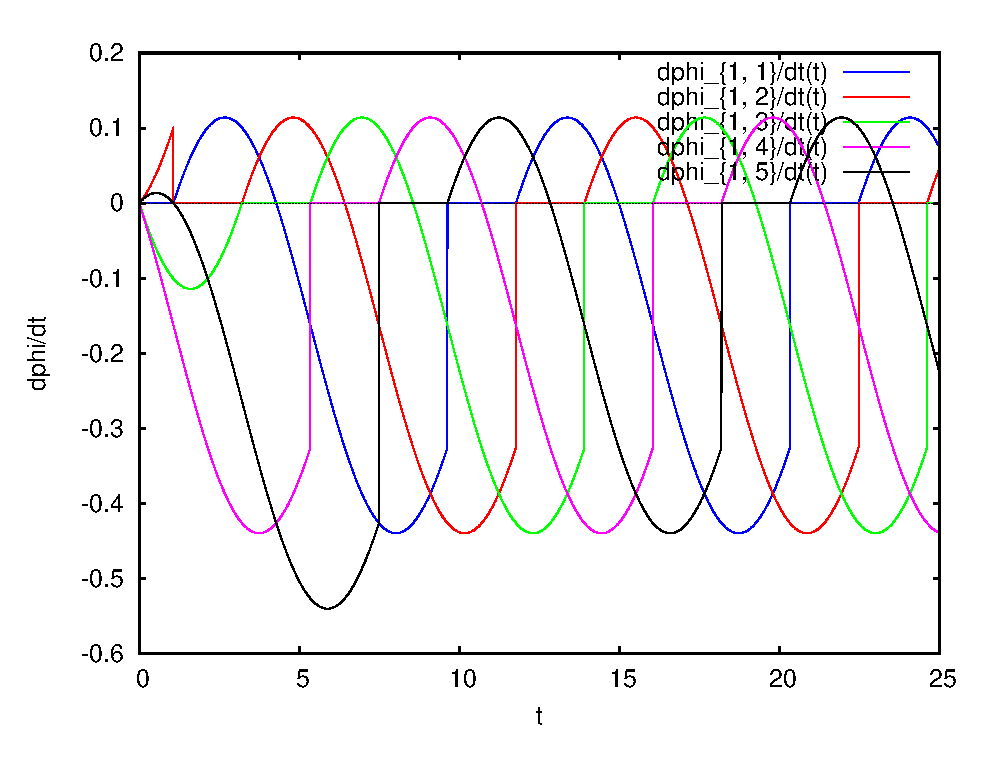
\includegraphics[width=\linewidth]{pic/rol__self_rot__velocities_of_rollers_of_wheel_1}
        \caption{Скорости роликов $\dot{\phi}_{ij}(t)$ на любом колесе}
        \label{fig:rol__self_rot__velocities_of_rollers_of_wheel_1}
    \end{subfigure}
    \begin{subfigure}[t]{0.3\textwidth}
        \centering
        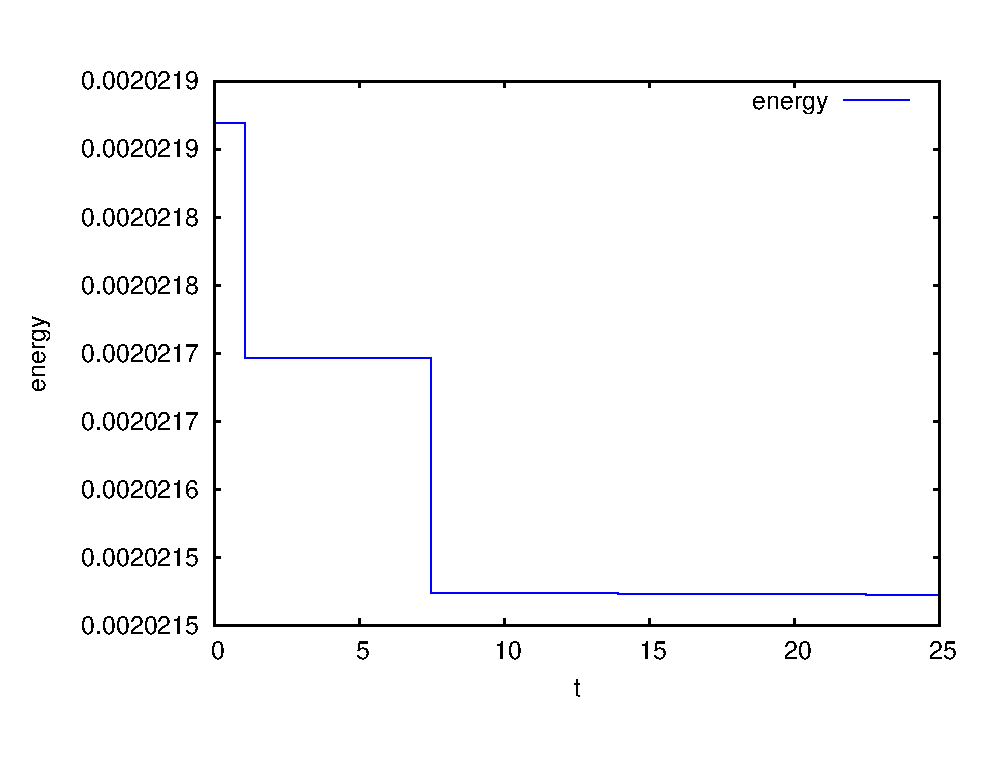
\includegraphics[width=\linewidth]{pic/rol__self_rot__kinetic_energy}
        \caption{Кинетическая энергия}
        \label{fig:rol__self_rot__kinetic_energy}    
    \end{subfigure}
    \begin{subfigure}[t]{0.3\textwidth}
        \centering
        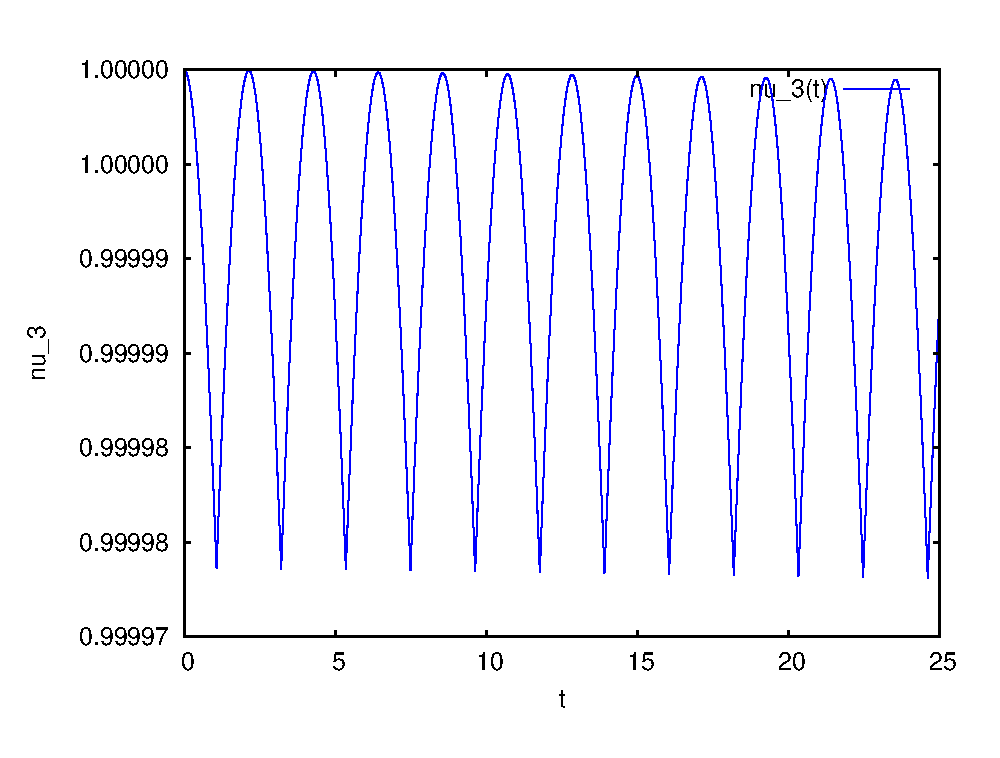
\includegraphics[width=\linewidth]{pic/rol__self_rot__velocity_of_self_rotation}
        \caption{Угловая скорость собственного вращения $\nu_3(t)$}
        \label{fig:rol__self_rot__velocity_of_self_rotation}    
    \end{subfigure}

    \caption{Экипаж с роликами. Вращение вокруг своей оси ($\nu_{1,2}(0) = 0, \nu_3 = 1$).}
    \label{fig:selfrot}
    
\end{figure}

\end{frame}

\begin{frame}{Движение по прямой ($\nu_1(0) = 1, \nu_{2,3} = 0$).}
    \begin{figure}[H]
    \centering

    \begin{columns}
        \column{0.45\textwidth}
            \centering
            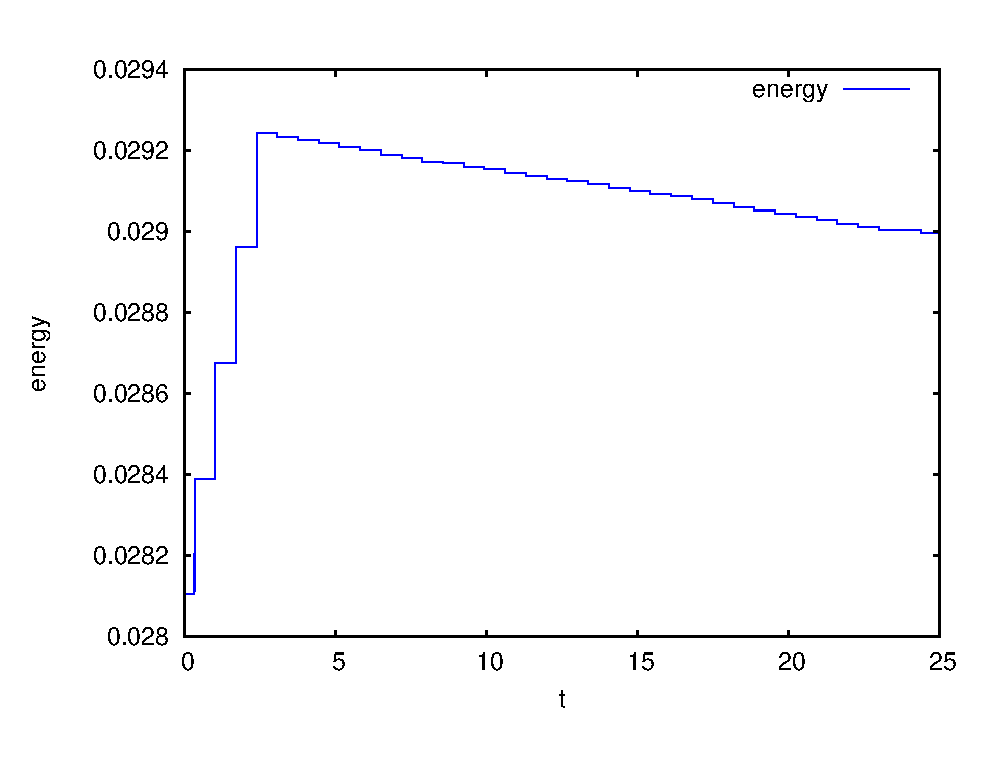
\includegraphics[width=\linewidth]{pic/rol__straight__kinetic_energy}\\
            Кинетическая энергия
        \column{0.45\textwidth}
            \centering
            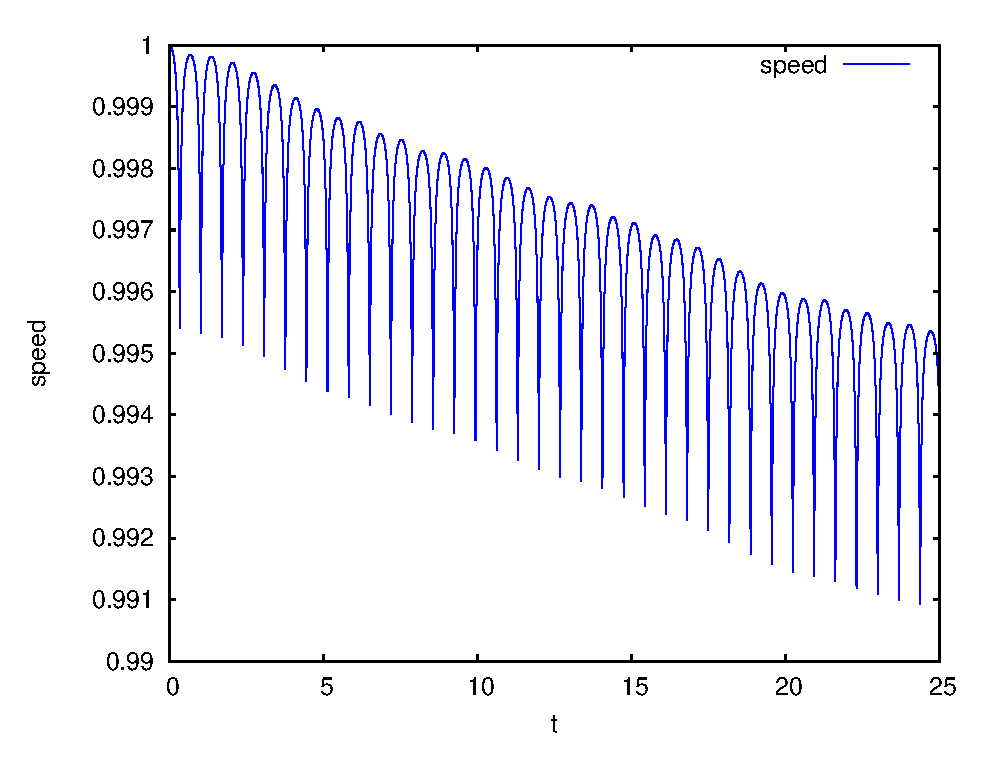
\includegraphics[width=\linewidth]{pic/rol__straight__speed_of_center_of_mass}\\
            Скорость центра масс
    \end{columns}
    
    \begin{columns}
        \column{0.35\textwidth}
            \centering
            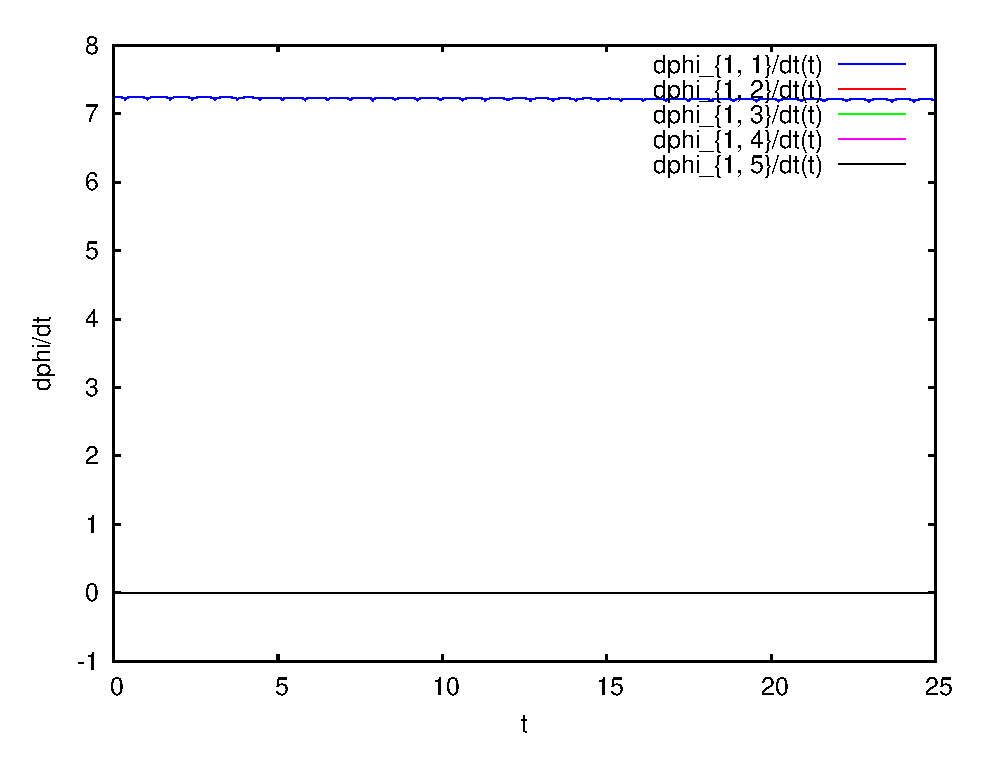
\includegraphics[width=\linewidth]{pic/rol__straight__velocities_of_rollers_of_wheel_1}\\
            $\dot{\phi}_{ij}(t)$ на переднем колесе
        \column{0.45\textwidth}
            \centering
            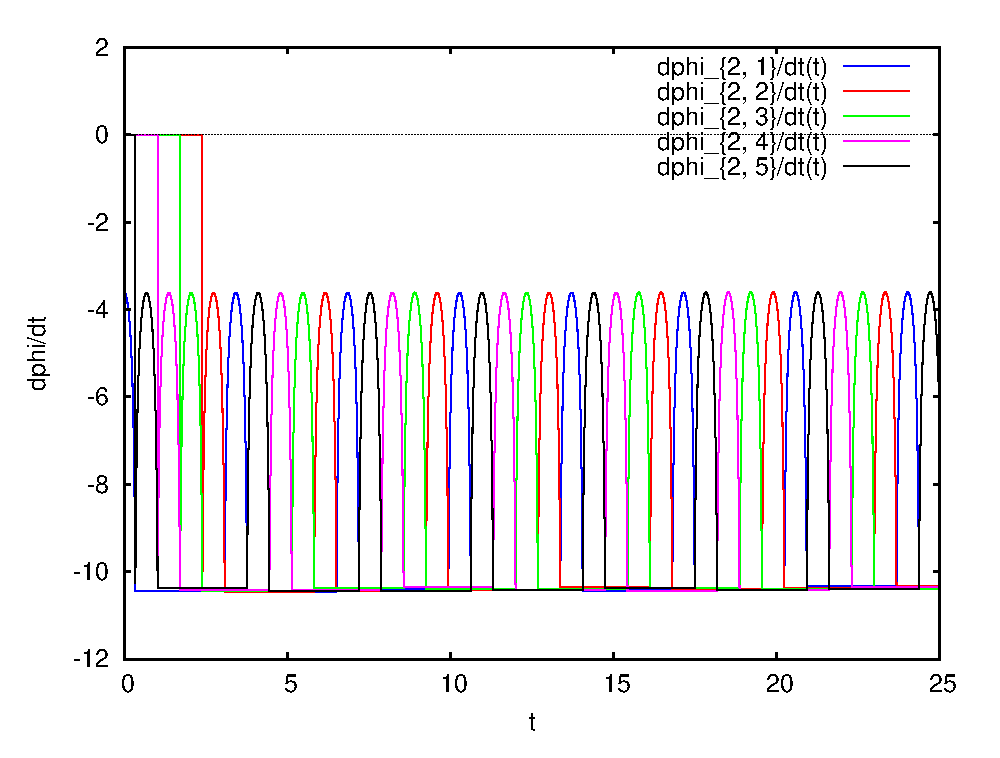
\includegraphics[width=\linewidth]{pic/rol__straight__velocities_of_rollers_of_wheel_2}\\
            $\dot{\phi}_{ij}(t)$ на правом заднем колесе
    \end{columns}

\end{figure}

\end{frame}

\begin{frame}{Движение с закруткой ($\nu_1(0) = 1, \nu_2(0) = 0, \nu_3(0) = 1$).}
    \begin{figure}
    \centering
    \begin{subfigure}[t]{0.45\textwidth}
        \centering
        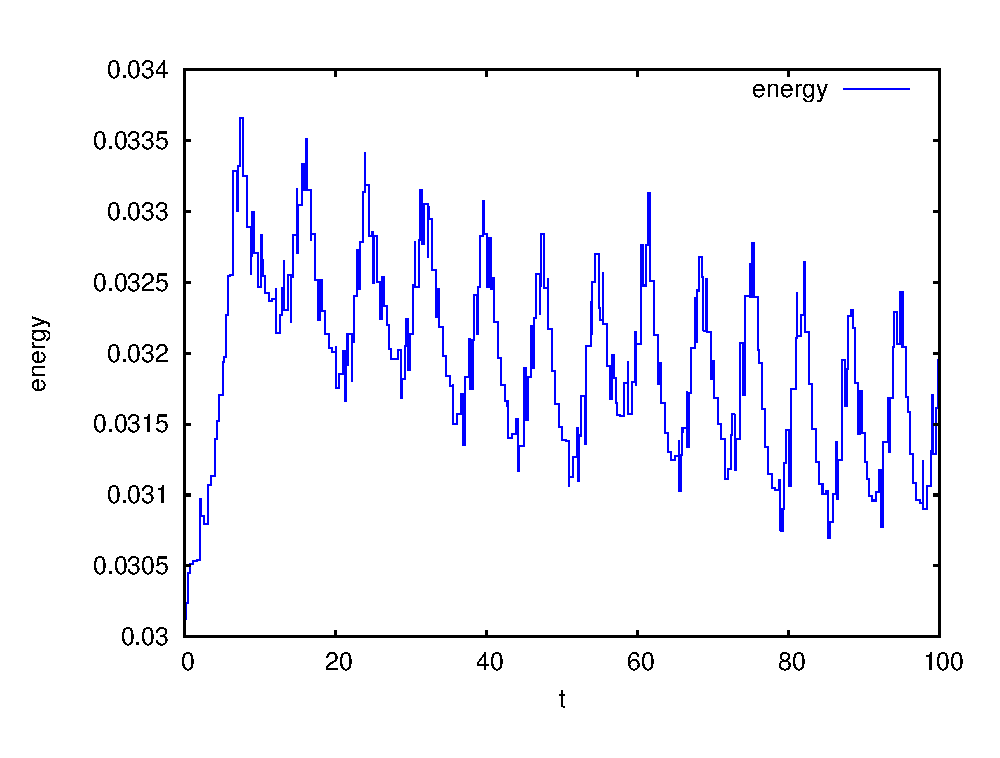
\includegraphics[width=\linewidth]{pic/rol__wrench__kinetic_energy}
        \caption{Кинетическая энергия}
        \label{fig:rol__wrench__kinetic_energy}
    \end{subfigure}
    \begin{subfigure}[t]{0.45\textwidth}
        \centering
        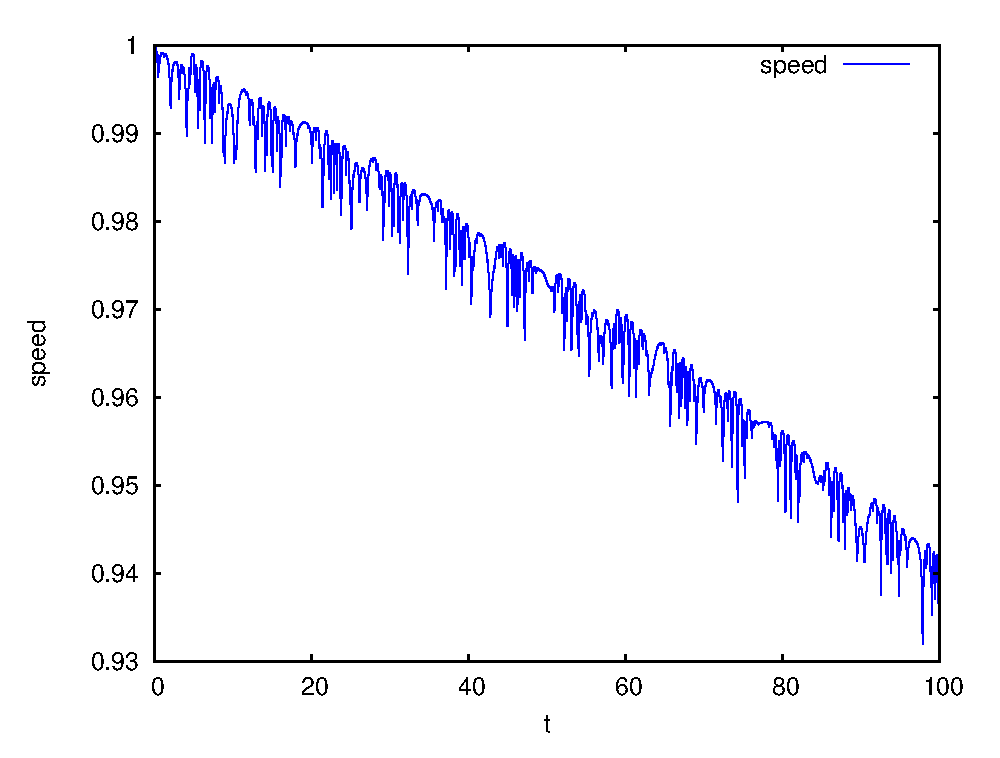
\includegraphics[width=\linewidth]{pic/rol__wrench__speed_of_center_of_mass}
        \caption{Скорость центра масс $\left(\nu_1^2 + \nu_2^2\right)(t)$}
        \label{fig:rol__wrench__speed_of_center_of_mass}
    \end{subfigure}
    \vspace{12pt}
    
    \begin{subfigure}[t]{0.45\textwidth}
        \centering
        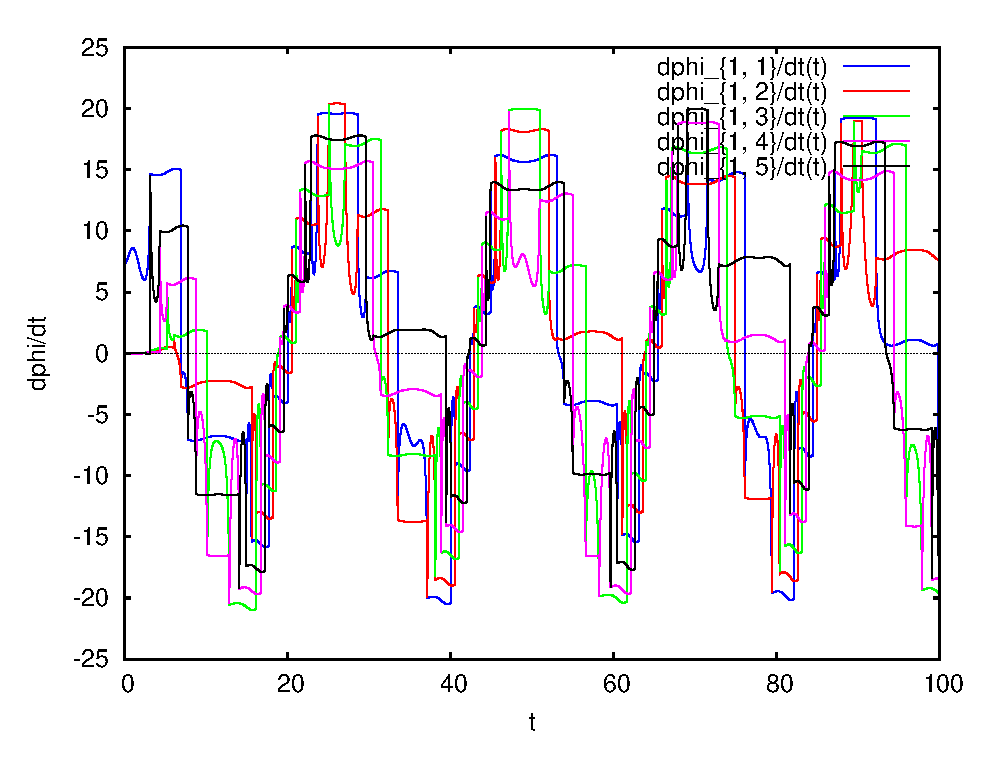
\includegraphics[width=\linewidth]{pic/rol__wrench__velocities_of_rollers_of_wheel_1}
        \caption{Скорости роликов $\dot{\phi}_{ij}(t)$ на первом колесе}
        \label{fig:rol__wrench__velocities_of_rollers_of_wheel_1}    
    \end{subfigure}
    \hfill
    \begin{subfigure}[t]{0.45\textwidth}
        \centering
        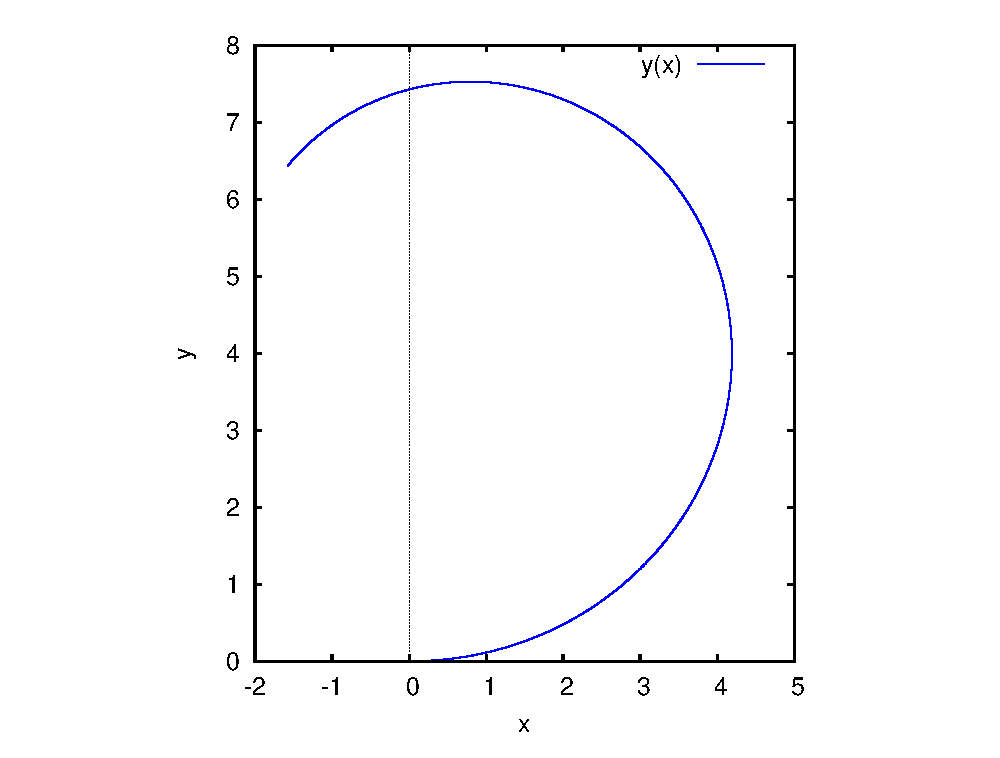
\includegraphics[width=\linewidth]{pic/rol__wrench__trajectory} \\
        \caption{Траектория центра масс на плоскости $OXY$}
        \label{fig:rol__wrench__trajectory}
    \end{subfigure}
    
    \caption{Экипаж c роликами. Движение с закруткой ($\nu_1(0) = 1, \nu_2(0) = 0, \nu_3(0) = 1$).}
    \label{fig:wrench}
    
\end{figure}

\end{frame}

% \begin{frame}{Вращение вокруг своей оси ($\nu_{1,2}(0) = 0, \nu_3 = 1$)}{Экипаж без роликов}
%     \begin{columns}
%         \column{0.33\textwidth}
%             \centering
%             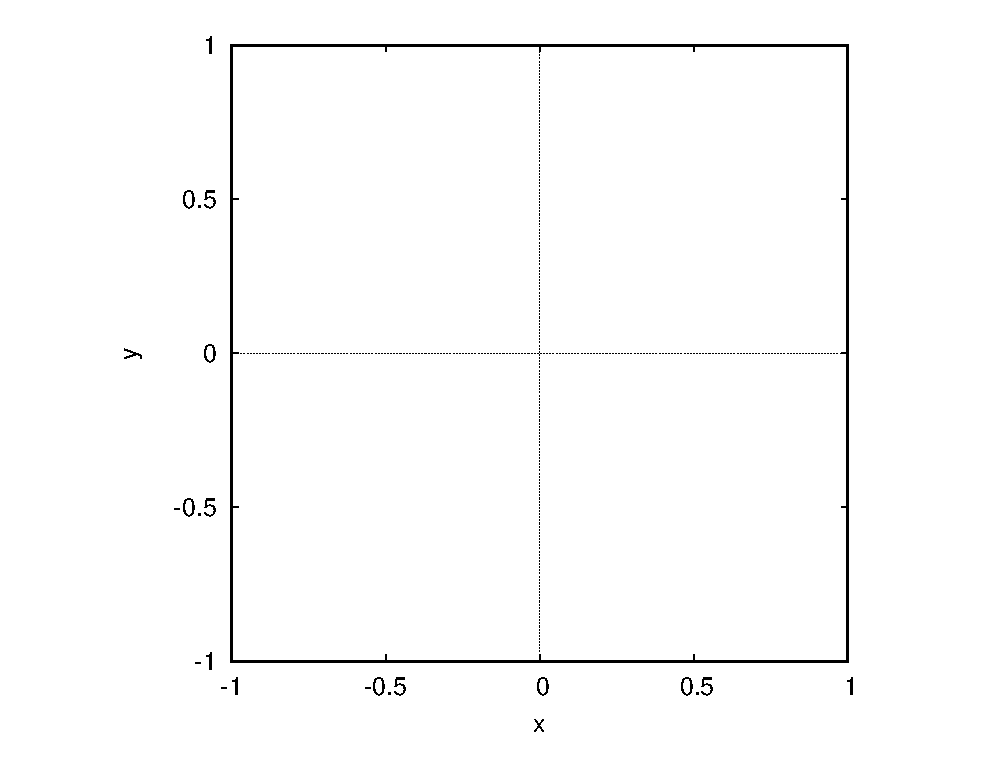
\includegraphics[width=\linewidth, height=30mm]{_old_sol__0_0_1__0__10__1e2_trajectory} \\
%             Траектория $X, Y$ \\
%             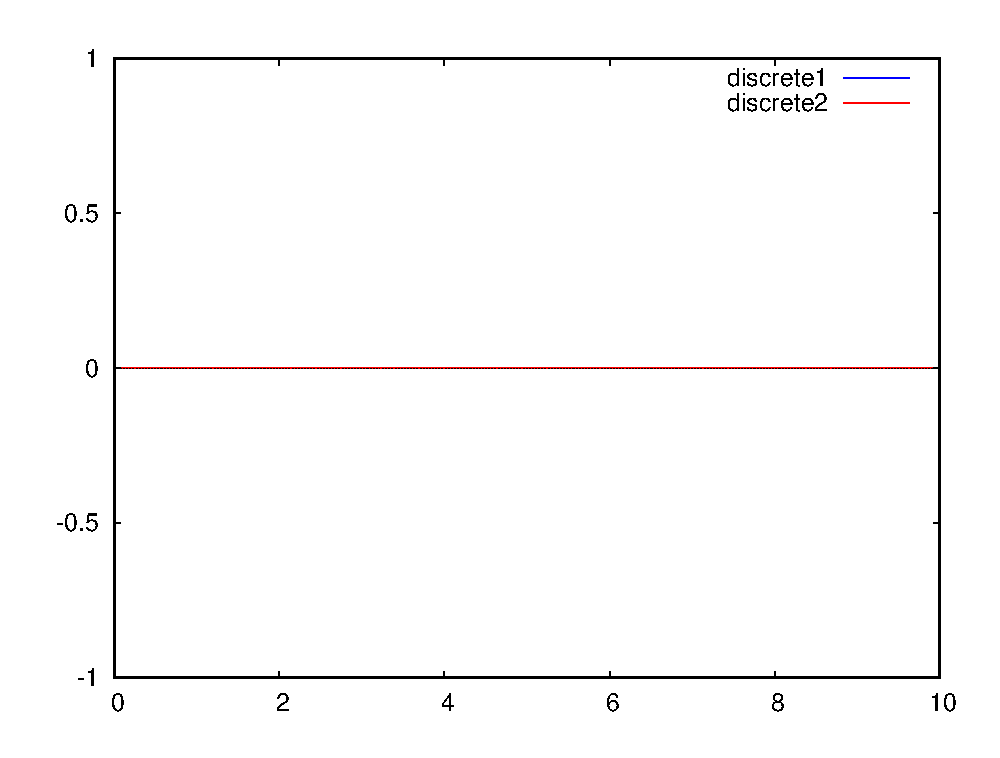
\includegraphics[width=\linewidth, height=30mm]{_old_sol__0_0_1__0__10__1e2_nu12} \\
%             $\nu_1(t), \nu_2(t)$
%         \column{0.33\textwidth}
%             \centering
%             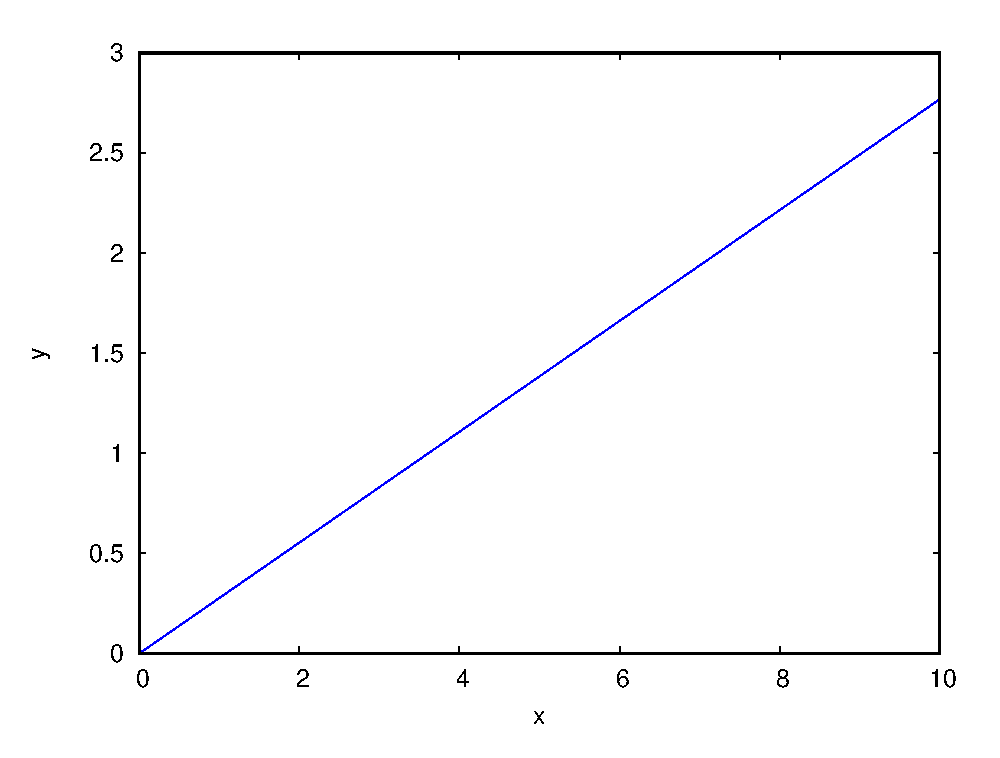
\includegraphics[width=\linewidth, height=30mm]{_old_sol__0_0_1__0__10__1e2_theta} \\
%             $\theta(t)$ \\
%             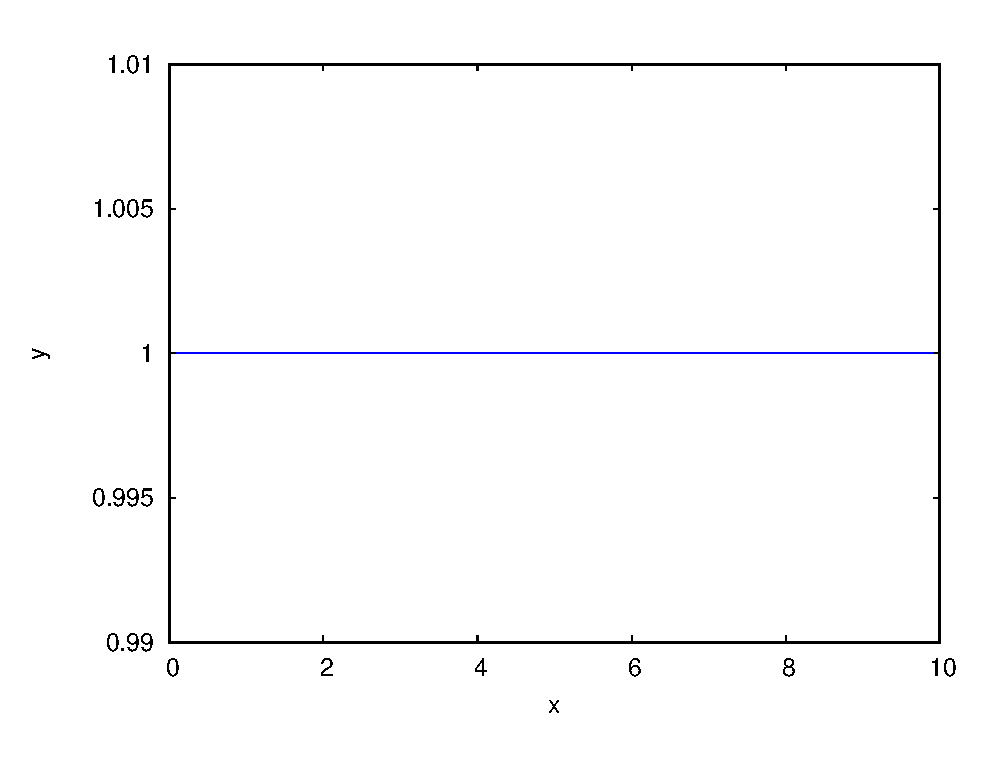
\includegraphics[width=\linewidth, height=30mm]{_old_sol__0_0_1__0__10__1e2_nu3} \\
%             $\nu_3(t)$
%         \column{0.33\textwidth}
%             \centering
%             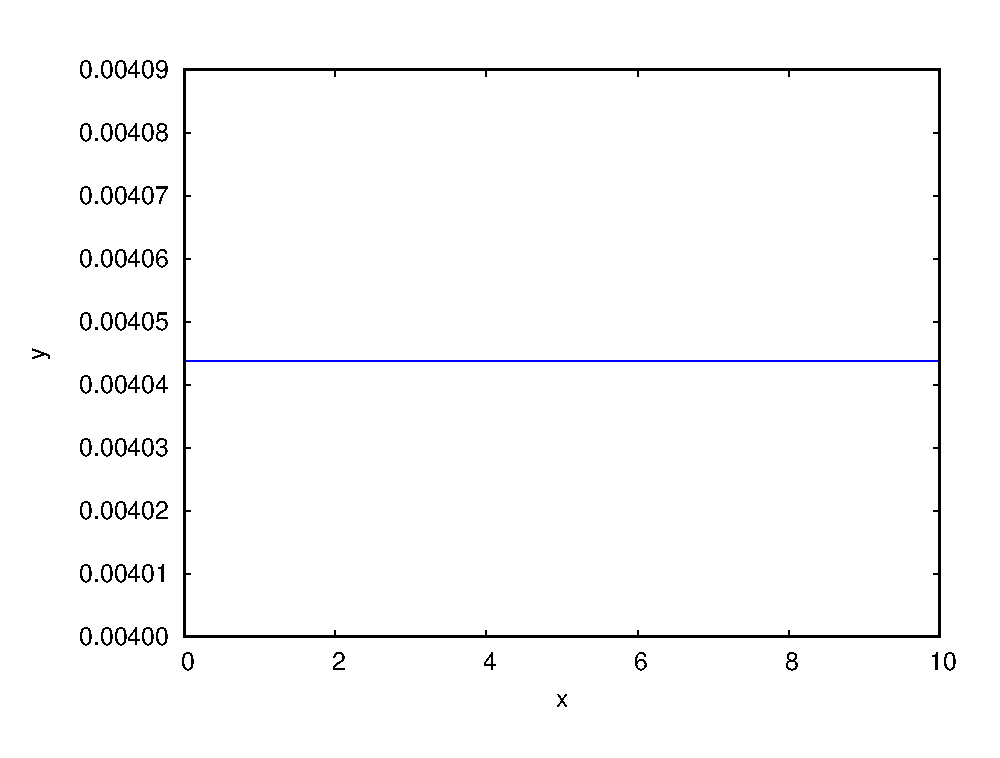
\includegraphics[width=\linewidth, height=30mm]{_old_sol__0_0_1__0__10__1e2_kin_en} \\
%             Кинетическая энергия \\
%             \vspace{15pt}
%             Центр экипажа неподвижен, скорость вращения и энергия постоянны.
%     \end{columns}
% \end{frame}

% \begin{frame}{Вращение вокруг своей оси ($\nu_{1,2}(0) = 0, \nu_3 = 1$)}{Экипаж с роликами}
%     \begin{columns}
%         \column{0.33\textwidth}
%             \centering
%             \includegraphics[width=\linewidth, height=30mm]{_sol__0_0_1__0__10__1e2_trajectory} \\
%             Траектория $X, Y$ \\
%             \includegraphics[width=\linewidth, height=30mm]{_sol__0_0_1__0__10__1e2_nu12} \\
%             $\nu_1(t), \nu_2(t)$
%         \column{0.33\textwidth}
%             \centering
%             \includegraphics[width=\linewidth, height=30mm]{_sol__0_0_1__0__10__1e2_theta} \\
%             $\theta(t)$ \\
%             \includegraphics[width=\linewidth, height=30mm]{_sol__0_0_1__0__10__1e2_nu3} \\
%             $\nu_3(t)$
%         \column{0.33\textwidth}
%             \centering
%             \includegraphics[width=\linewidth, height=30mm]{_sol__0_0_1__0__10__1e2_kin_en} \\
%             Кинетическая энергия \\
%             \vspace{15pt}
%             Идентично случаю с роликами.
%     \end{columns}
% \end{frame}

% \begin{frame}{Движение по прямой ($\nu_1(0) = 1, \nu_{2,3} = 0$)}{Экипаж без роликов}
%     \begin{columns}
%         \column{0.33\textwidth}
%             \centering
%             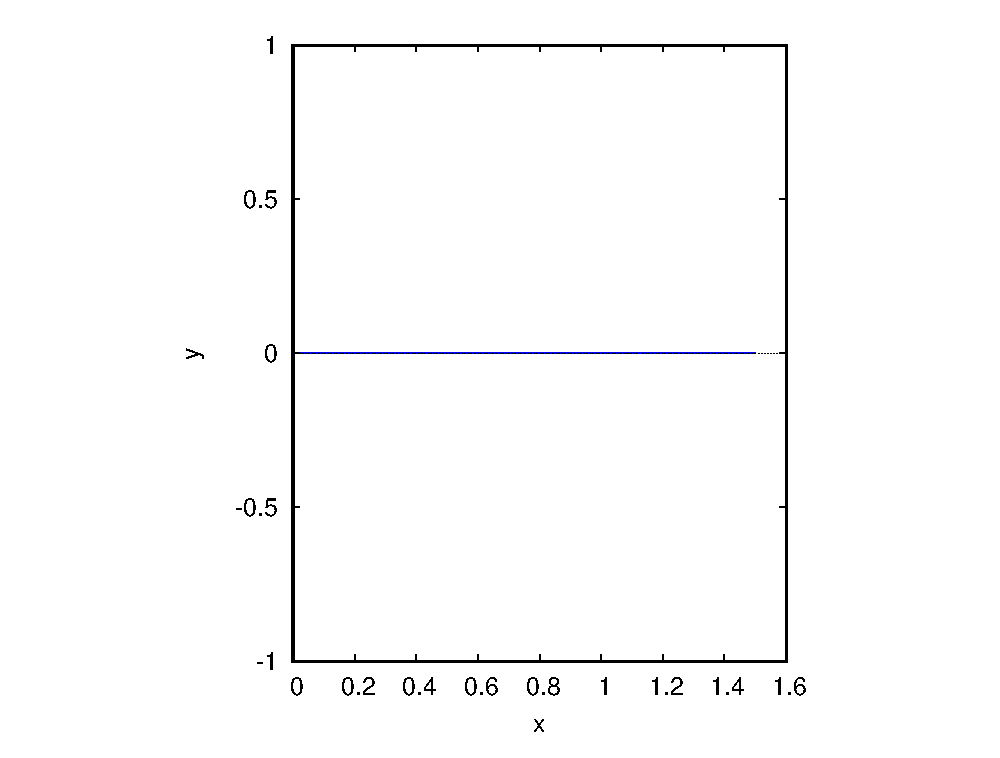
\includegraphics[width=\linewidth, height=30mm]{_old_sol__1_0_0__0__10__1e2_trajectory} \\
%             Траектория $X, Y$ \\
%             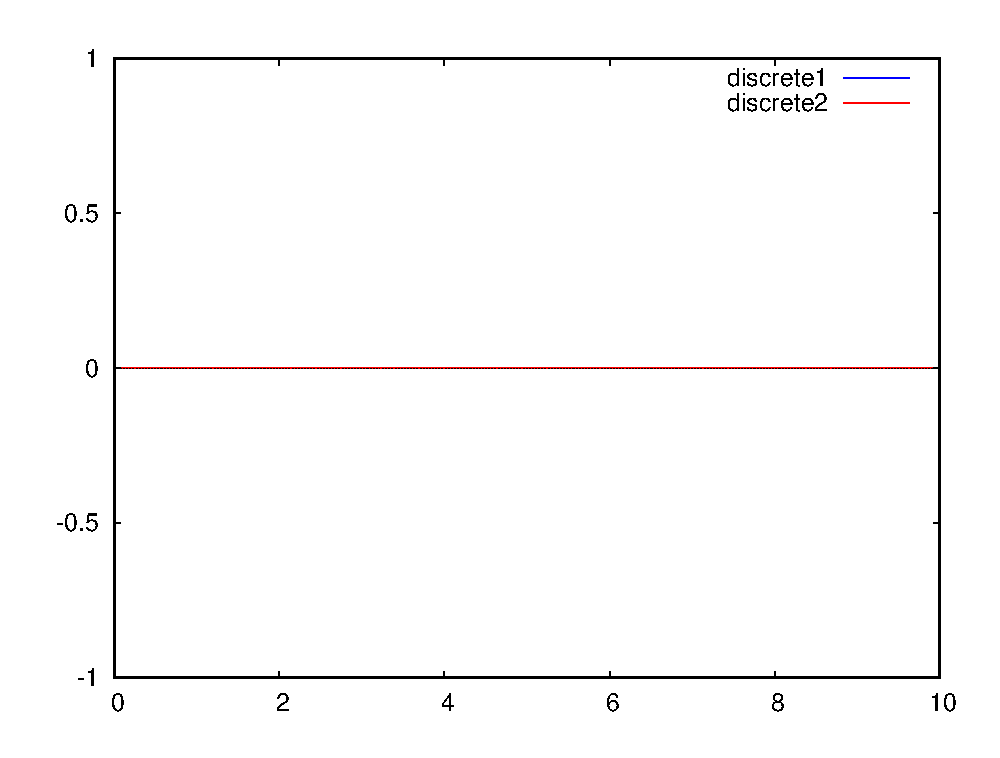
\includegraphics[width=\linewidth, height=30mm]{_old_sol__1_0_0__0__10__1e2_nu12_centered} \\
%             $\nu_{1,2}(t) - \nu_{1,2}(0)$
%         \column{0.33\textwidth}
%             \centering
%             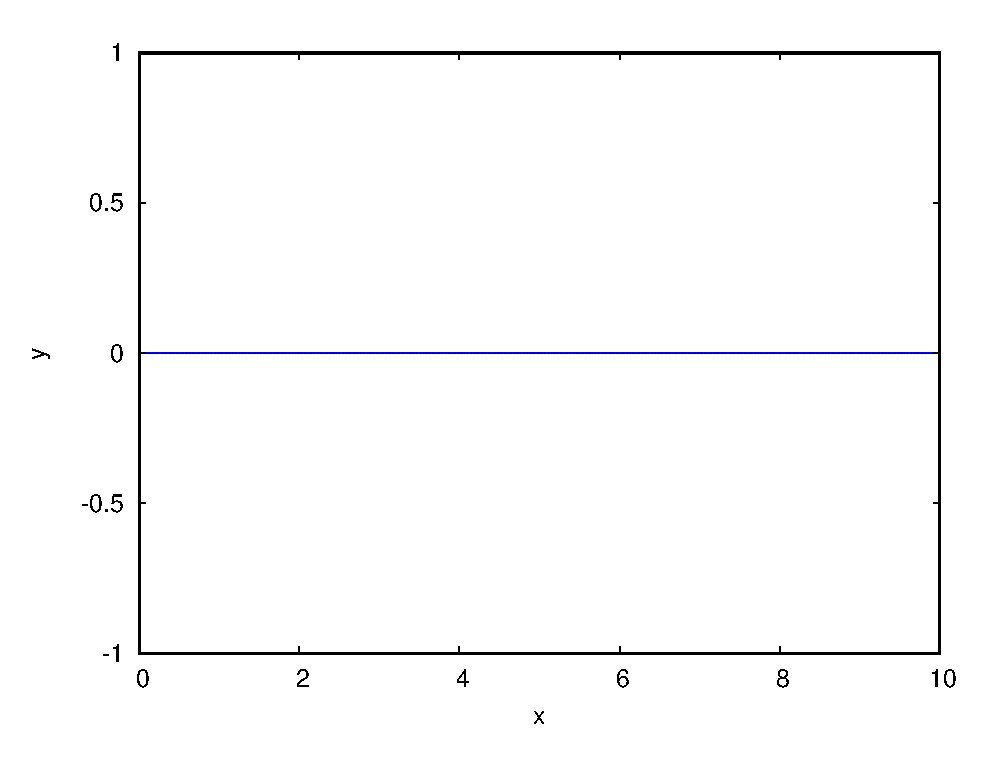
\includegraphics[width=\linewidth, height=30mm]{_old_sol__1_0_0__0__10__1e2_theta} \\
%             $\theta(t)$ \\
%             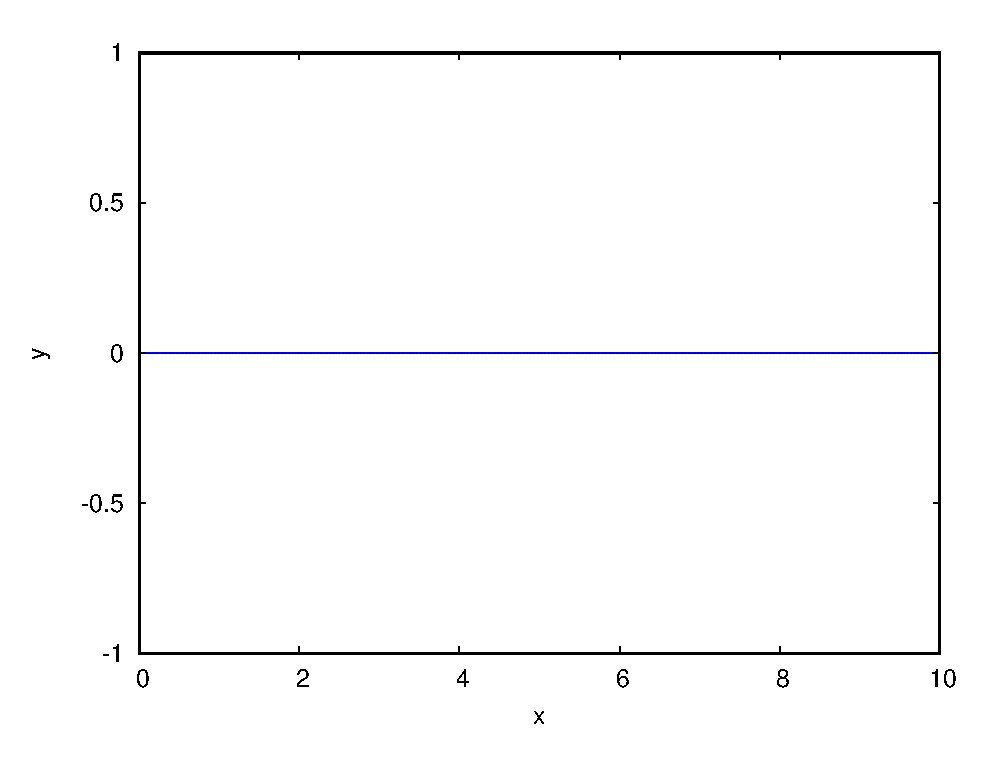
\includegraphics[width=\linewidth, height=30mm]{_old_sol__1_0_0__0__10__1e2_nu3} \\
%             $\nu_3(t)$
%         \column{0.33\textwidth}
%             \centering
%             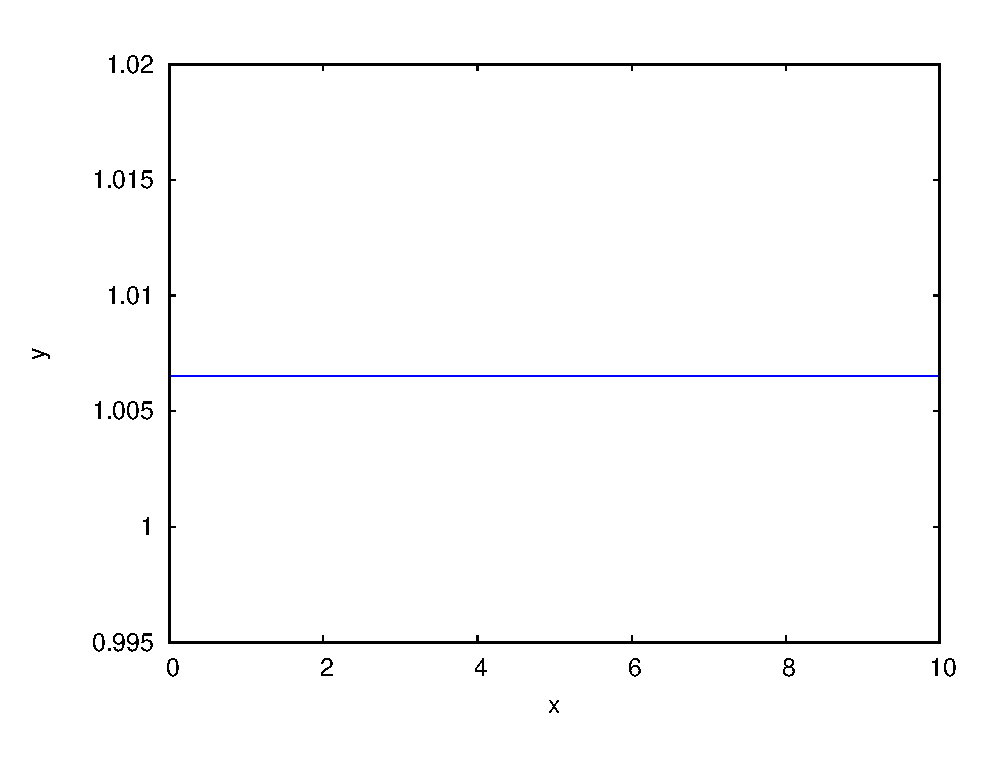
\includegraphics[width=\linewidth, height=30mm]{_old_sol__1_0_0__0__10__1e2_kin_en} \\
%             Кинетическая энергия \\
%             \vspace{15pt}
%             Экипаж равномерно движется по прямой, не вращаясь, энергия постоянна.
%     \end{columns}
% \end{frame}

% \begin{frame}{Движение по прямой ($\nu_1(0) = 1, \nu_{2,3} = 0$)}{Экипаж с роликами}
%     \begin{columns}
%         \column{0.33\textwidth}
%             \centering
%             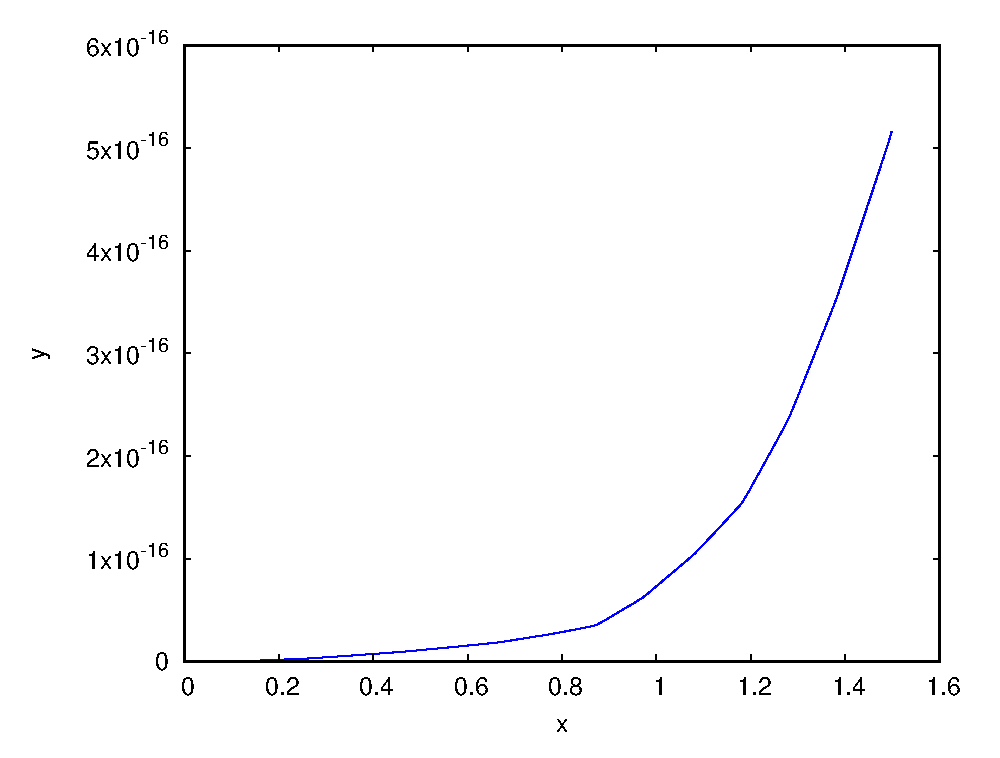
\includegraphics[width=\linewidth, height=30mm]{_sol__1_0_0__0__10__1e2_trajectory} \\
%             Траектория $X, Y$ \\
%             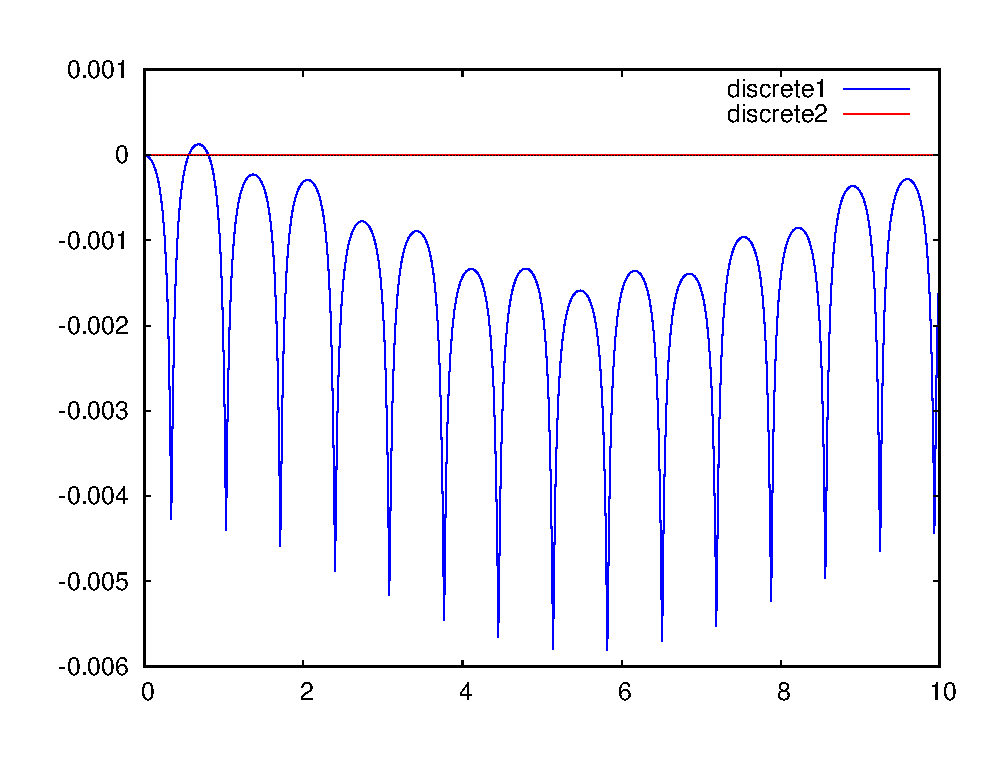
\includegraphics[width=\linewidth, height=30mm]{_sol__1_0_0__0__10__1e2_nu12_centered} \\
%             $\nu_{1,2}(t) - \nu_{1,2}(0)$
%         \column{0.33\textwidth}
%             \centering
%             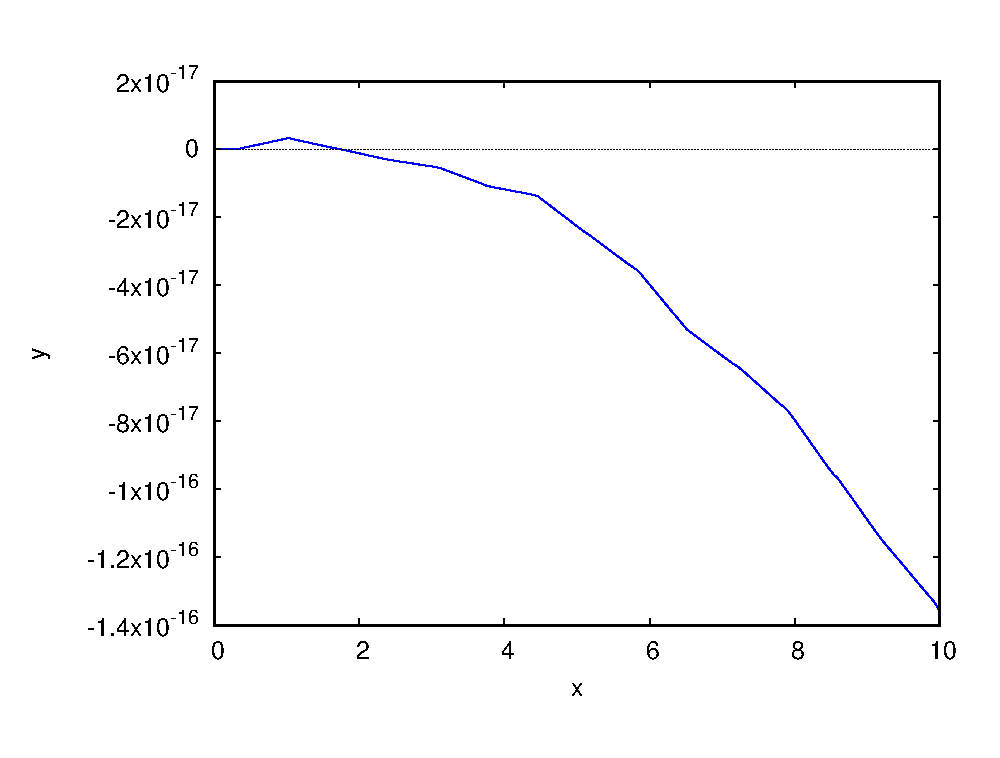
\includegraphics[width=\linewidth, height=30mm]{_sol__1_0_0__0__10__1e2_theta} \\
%             $\theta(t)$ \\
%             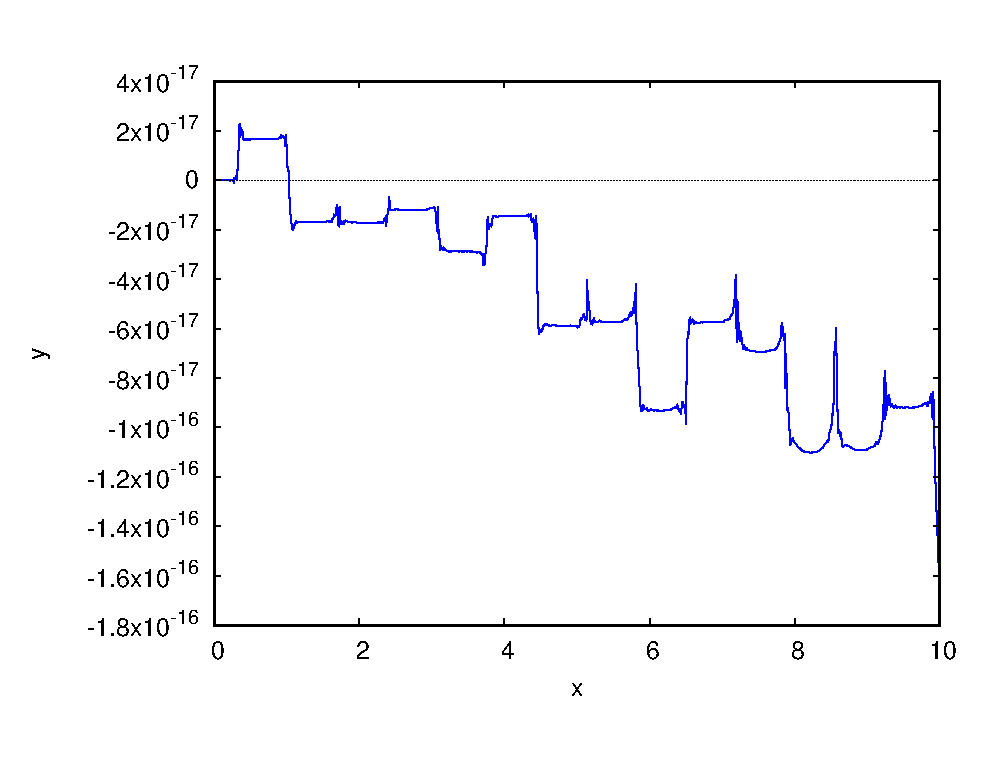
\includegraphics[width=\linewidth, height=30mm]{_sol__1_0_0__0__10__1e2_nu3} \\
%             $\nu_3(t)$
%         \column{0.33\textwidth}
%             \centering
%             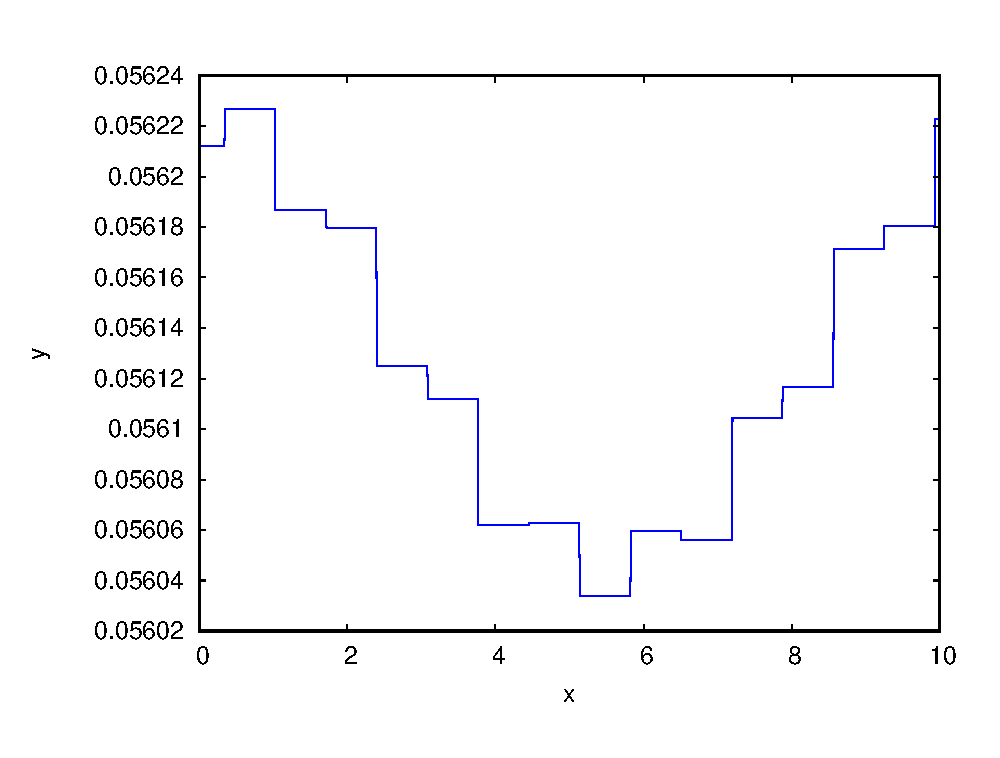
\includegraphics[width=\linewidth, height=30mm]{_sol__1_0_0__0__10__1e2_kin_en} \\
%             Кинетическая энергия \\
%             \vspace{15pt}
%             Энергия и псевдоскорость $\nu_1$ не постоянны. Присутствует шум по координатам.
%     \end{columns}
% \end{frame}

% \begin{frame}{Движение с закруткой ($\nu_1(0) = 1, \nu_2(0) = 0, \nu_3(0) = 1$)}{Экипаж без роликов}
%     \begin{columns}
%         \column{0.33\textwidth}
%             \centering
%             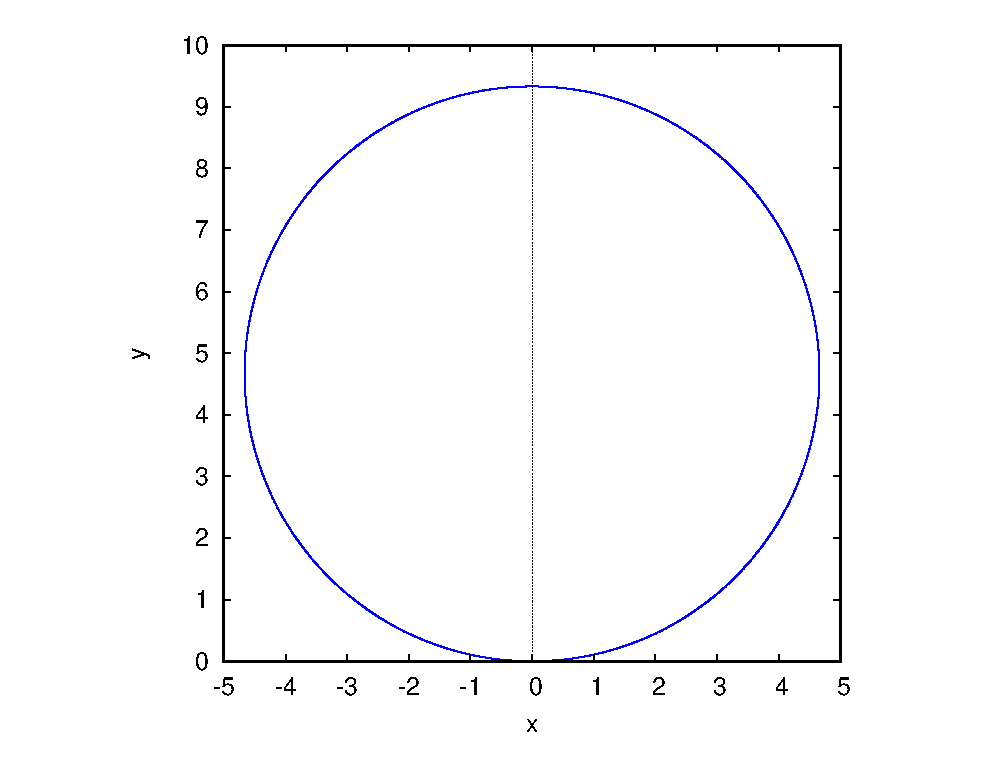
\includegraphics[width=\linewidth, height=30mm]{_old_sol__1_0_1__0__230__1e2_trajectory} \\
%             Траектория $X, Y$ \\
%             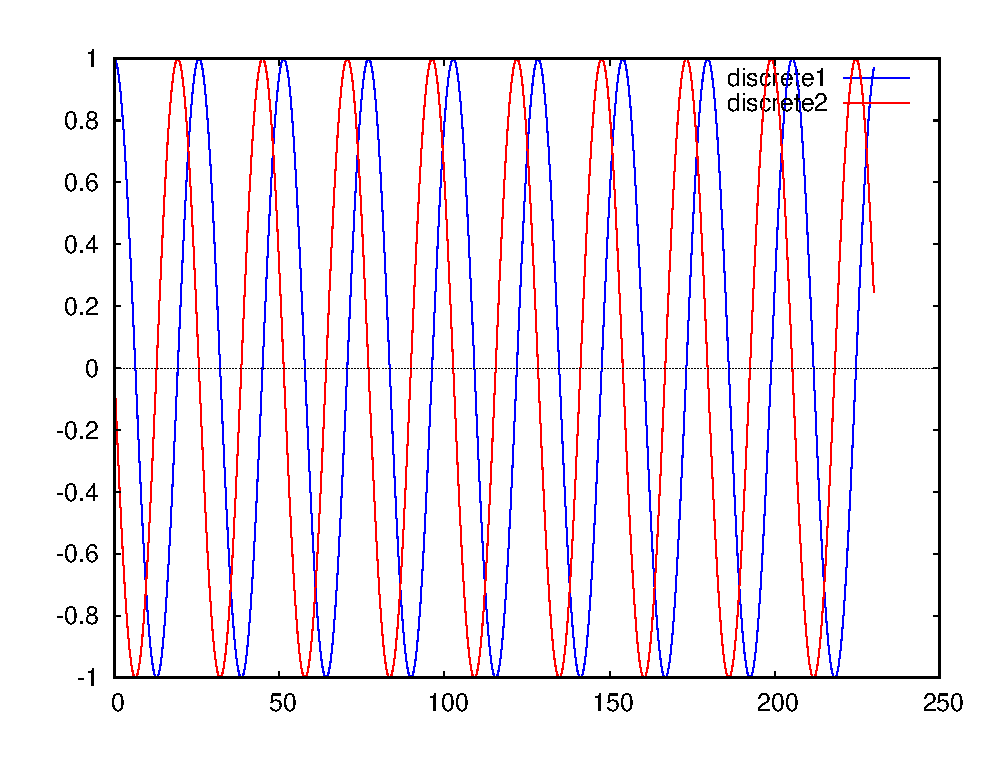
\includegraphics[width=\linewidth, height=30mm]{_old_sol__1_0_1__0__230__1e2_nu12} \\
%             $\nu_{1,2}(t) - \nu_{1,2}(0)$
%         \column{0.33\textwidth}
%             \centering
%             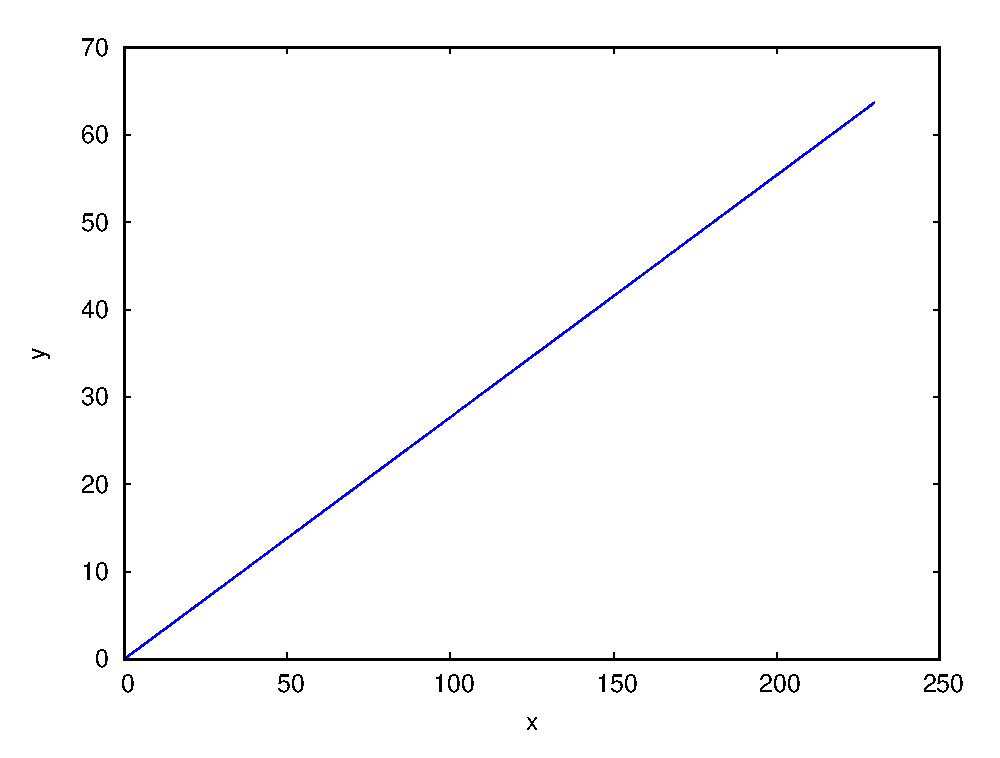
\includegraphics[width=\linewidth, height=30mm]{_old_sol__1_0_1__0__230__1e2_theta} \\
%             $\theta(t)$ \\
%             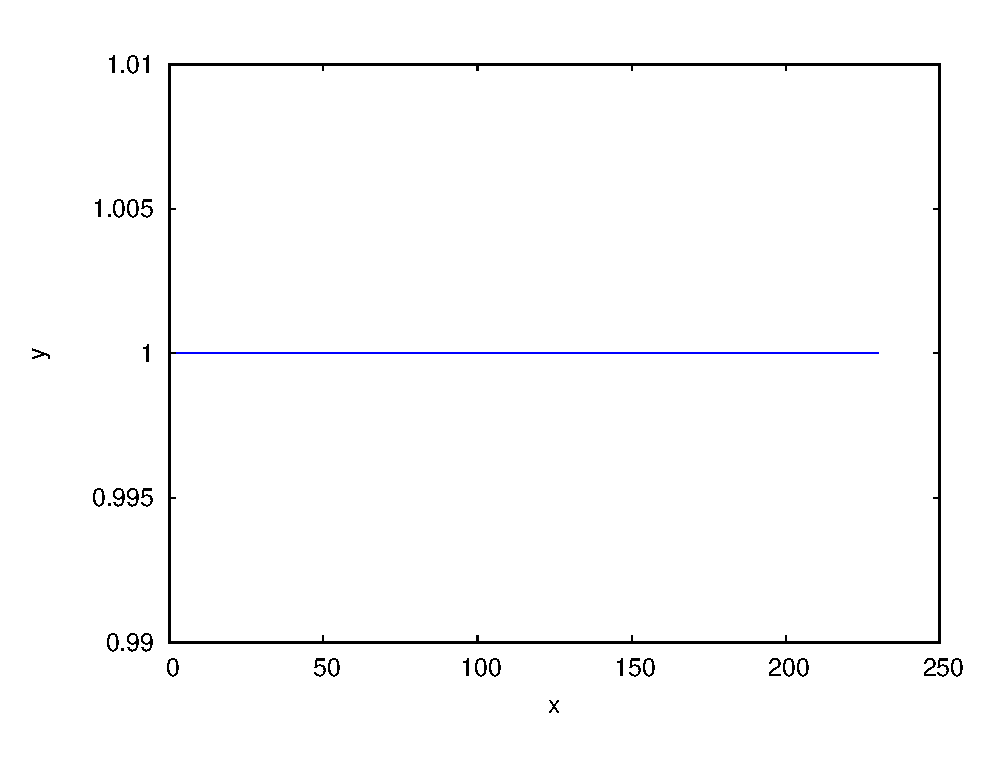
\includegraphics[width=\linewidth, height=30mm]{_old_sol__1_0_1__0__230__1e2_nu3} \\
%             $\nu_3(t)$
%         \column{0.33\textwidth}
%             \centering
%             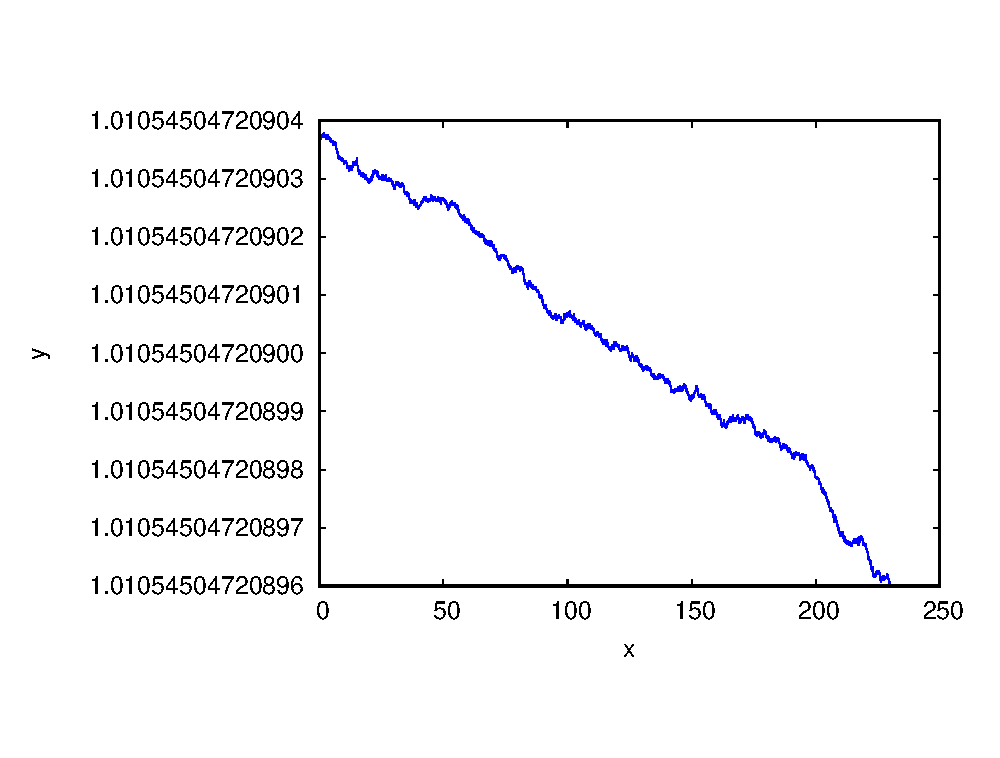
\includegraphics[width=\linewidth, height=30mm]{_old_sol__1_0_1__0__230__1e2_kin_en} \\
%             Кинетическая энергия \\
%             \vspace{15pt}
%             Экипаж движется по окружности, равномерно вращаясь вокруг своей оси.
%     \end{columns}
% \end{frame}

% \begin{frame}{Движение с закруткой ($\nu_1(0) = 1, \nu_2(0) = 0, \nu_3(0) = 1$)}{Экипаж c роликами}
%     \begin{columns}
%         \column{0.33\textwidth}
%             \centering
%             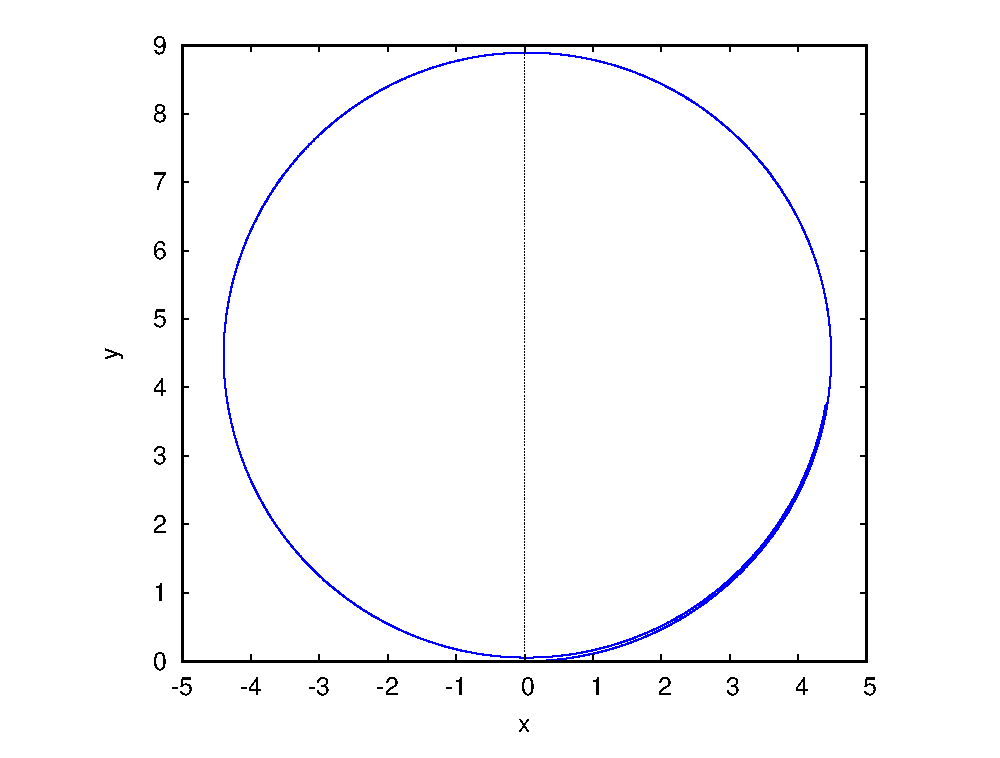
\includegraphics[width=\linewidth, height=30mm]{_sol__1_0_1__0__230__1e2_trajectory} \\
%             Траектория $X, Y$ \\
%             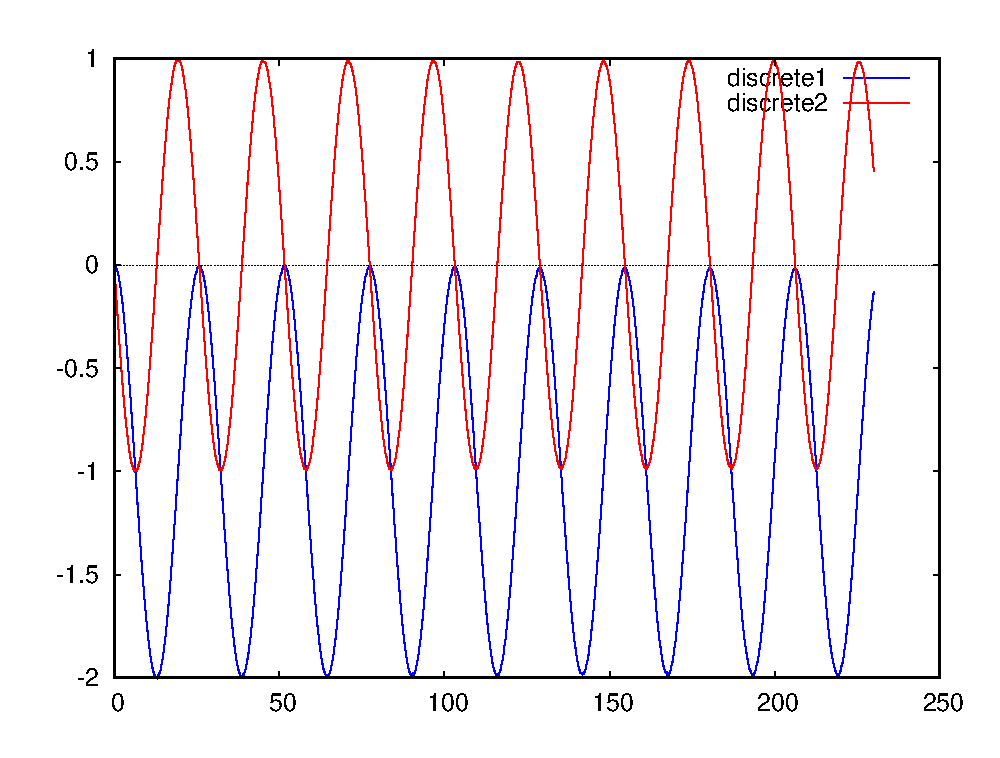
\includegraphics[width=\linewidth, height=30mm]{_sol__1_0_1__0__230__1e2_nu12_centered} \\
%             $\nu_{1,2}(t) - \nu_{1,2}(0)$
%         \column{0.33\textwidth}
%             \centering
%             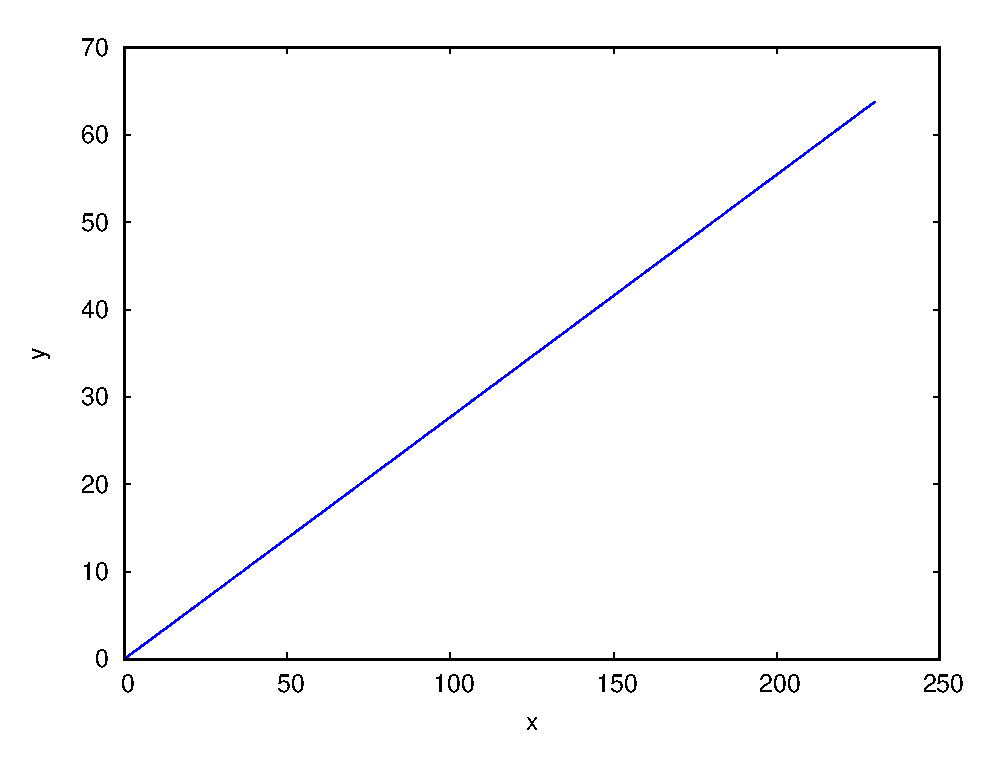
\includegraphics[width=\linewidth, height=30mm]{_sol__1_0_1__0__230__1e2_theta} \\
%             $\theta(t)$ \\
%             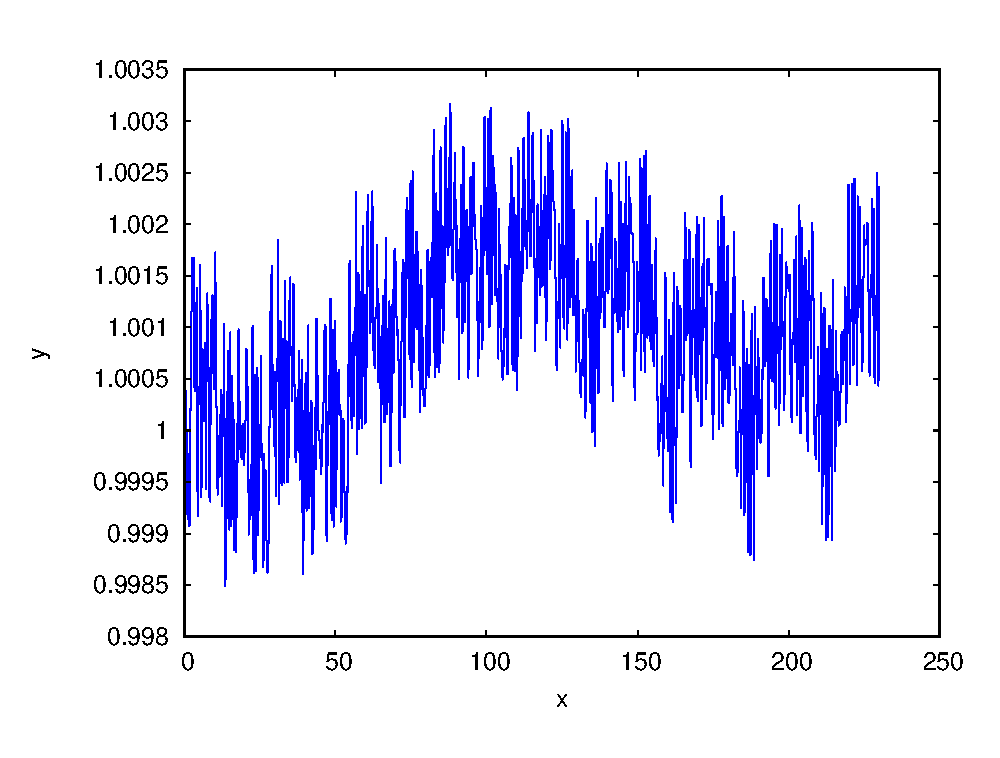
\includegraphics[width=\linewidth, height=30mm]{_sol__1_0_1__0__230__1e2_nu3} \\
%             $\nu_3(t)$
%         \column{0.33\textwidth}
%             \centering
%             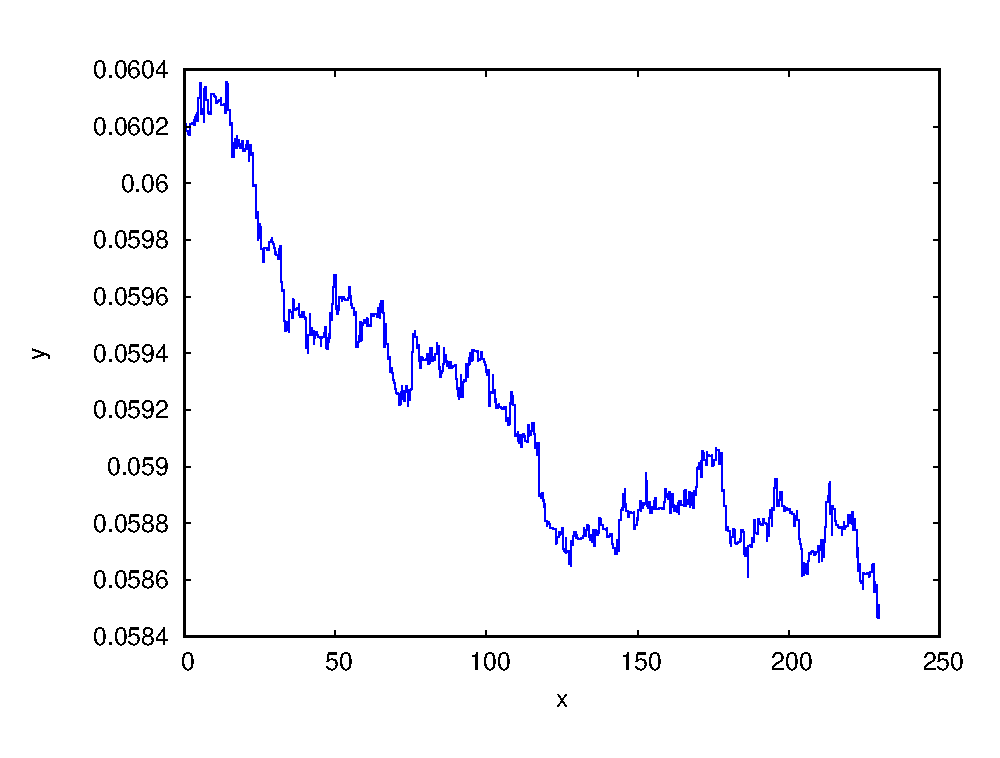
\includegraphics[width=\linewidth, height=30mm]{_sol__1_0_1__0__230__1e2_kin_en} \\
%             Кинетическая энергия \\
%             \vspace{15pt}
%             Энергия не постоянна. Биения в псевдоскоростях.
%     \end{columns}
% \end{frame}

% \begin{frame}{Движение с закруткой ($\nu_1(0) = 1, \nu_2(0) = 0, \nu_3(0) = 1$)}{Экипаж c роликами}
%     \begin{columns}
%         \column{0.33\textwidth}
%             \centering
%             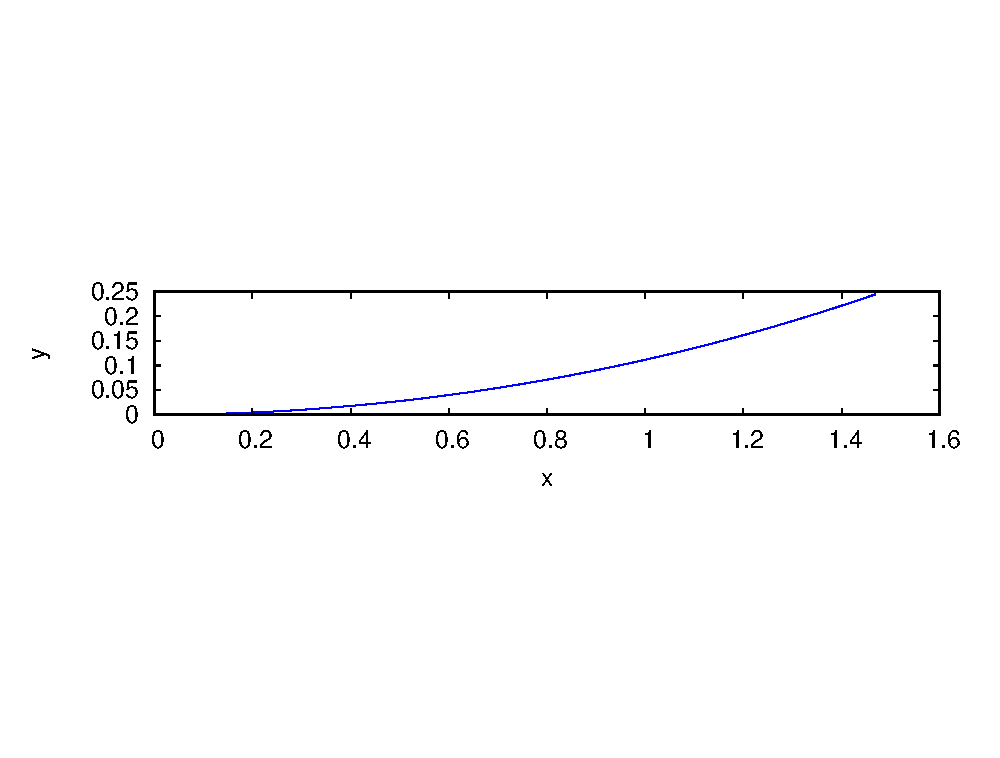
\includegraphics[width=\linewidth, height=30mm]{_sol__1_0_1__0__10__1e2_trajectory} \\
%             Траектория $X, Y$ \\
%             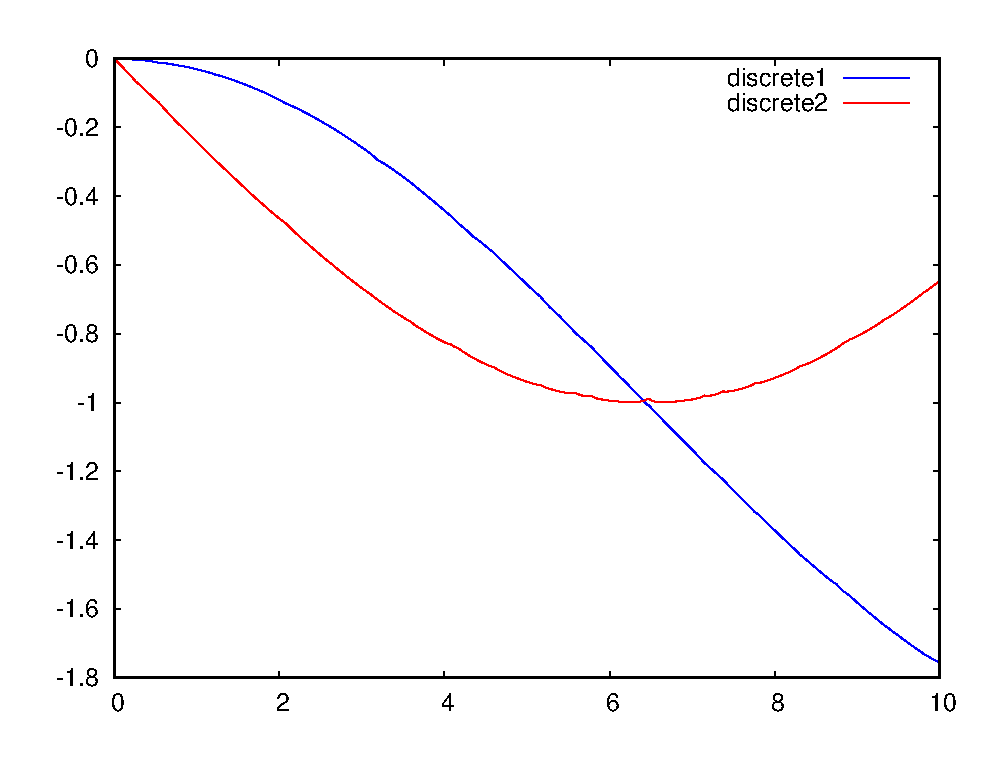
\includegraphics[width=\linewidth, height=30mm]{_sol__1_0_1__0__10__1e2_nu12_centered} \\
%             $\nu_{1,2}(t) - \nu_{1,2}(0)$
%         \column{0.33\textwidth}
%             \centering
%             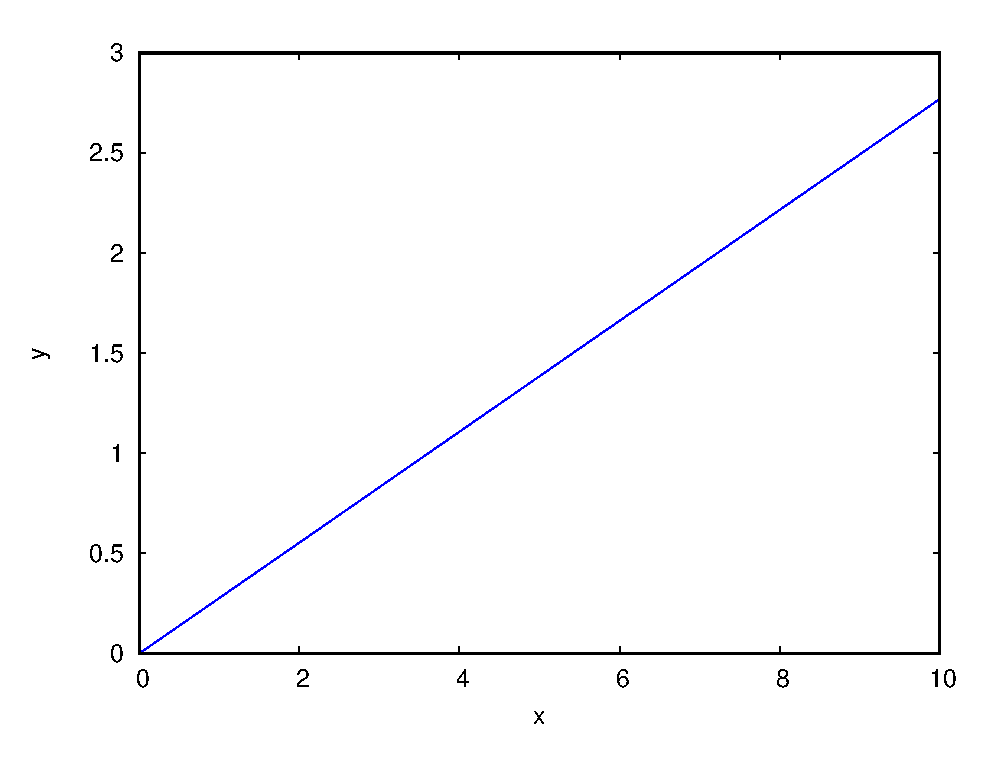
\includegraphics[width=\linewidth, height=30mm]{_sol__1_0_1__0__10__1e2_theta} \\
%             $\theta(t)$ \\
%             \includegraphics[width=\linewidth, height=30mm]{_sol__1_0_1__0__10__1e2_nu3} \\
%             $\nu_3(t)$
%         \column{0.33\textwidth}
%             \centering
%             \includegraphics[width=\linewidth, height=30mm]{_sol__1_0_1__0__10__1e2_kin_en} \\
%             Кинетическая энергия \\
%             \vspace{15pt}
%             Энергия не постоянна. Биения в псевдоскоростях.
%     \end{columns}
% \end{frame}

\begin{frame}{Результаты}
  \begin{itemize}
  \item
    Получены уравнения движения экипажа \alert{с полным набором роликов} в неголономной постановке.
  \item
    Показано, что разница с уравнениями для системы без роликов пропорциональна моменту инерции ролика.
  \item
    Выявлены свойства движения и первые интегралы.
  \item \alert{Учтено движение свободных роликов} и обнаружено его существенное влияние.
  \item
    Получены численные решения для симметричной конфигурации.
  \end{itemize}
  \vspace{10pt}
  \centering
  \textcolor{Periwinkle}{Спасибо за внимание!}
\end{frame}

\end{document}


